\chapter{Evaluation of temperature effects on ASIC performance} \label{ch1}

This Chapter describes the characterisation activity that has been carried out on the SLIDER32 ASIC employed for the readout of the lithium-drifted silicon, Si(Li), detectors of the GAPS inner tracker, described in \hyperref[gapsTrackingSystem]{Appendix \ref{gapsTrackingSystem}}. Specifically, the measurements were taken with a purposely developed test board described in \hyperref[testboardsetup]{Section \ref{testboardsetup}} and were aimed at the evaluation of thermal effects on:

\begin{enumerate}
    %\bfseries
    \itemsep0em 
    \item Bandgap reference current.
    \item Channel input-output characteristic.
    \item Digital-to-Analog Converter (DAC) used to set the global threshold voltage.
\end{enumerate}

\par
The characterisation activity has also been focused on the evaluation of electronic noise performance of the readout channel in the form of Equivalent Noise Charge (ENC), measured at a temperature of \SI{-40}{\celsius}, that is, the temperature at which the readout electronics will work during the experiment \cite{re_2022_a}, therefore a precise evaluation of the noise contribution at this temperature is of fundamental importance.

%-------------------------------------------------------------------------------
%	Test setup description and characterisation process
%-------------------------------------------------------------------------------

\section[Test setup description and characterisation process]{Test setup description and characterisation\\ process} \label{testboardsetup}

The setup used for the temperature characterisation of the SLIDER32 ASIC has been designed in two variants, which only differ on one component, namely an Agilent 34461A digital multimeter in version \texttt{1}, shown in \hyperref[figTESTBOARDsetup1]{Figure \ref{figTESTBOARDsetup1}}, in place of a Keysight E3631A DC power supply in version \texttt{2}, shown in \hyperref[figTESTBOARDsetup2]{Figure \ref{figTESTBOARDsetup2}}.

\begin{figure}[ht]
    \centering
    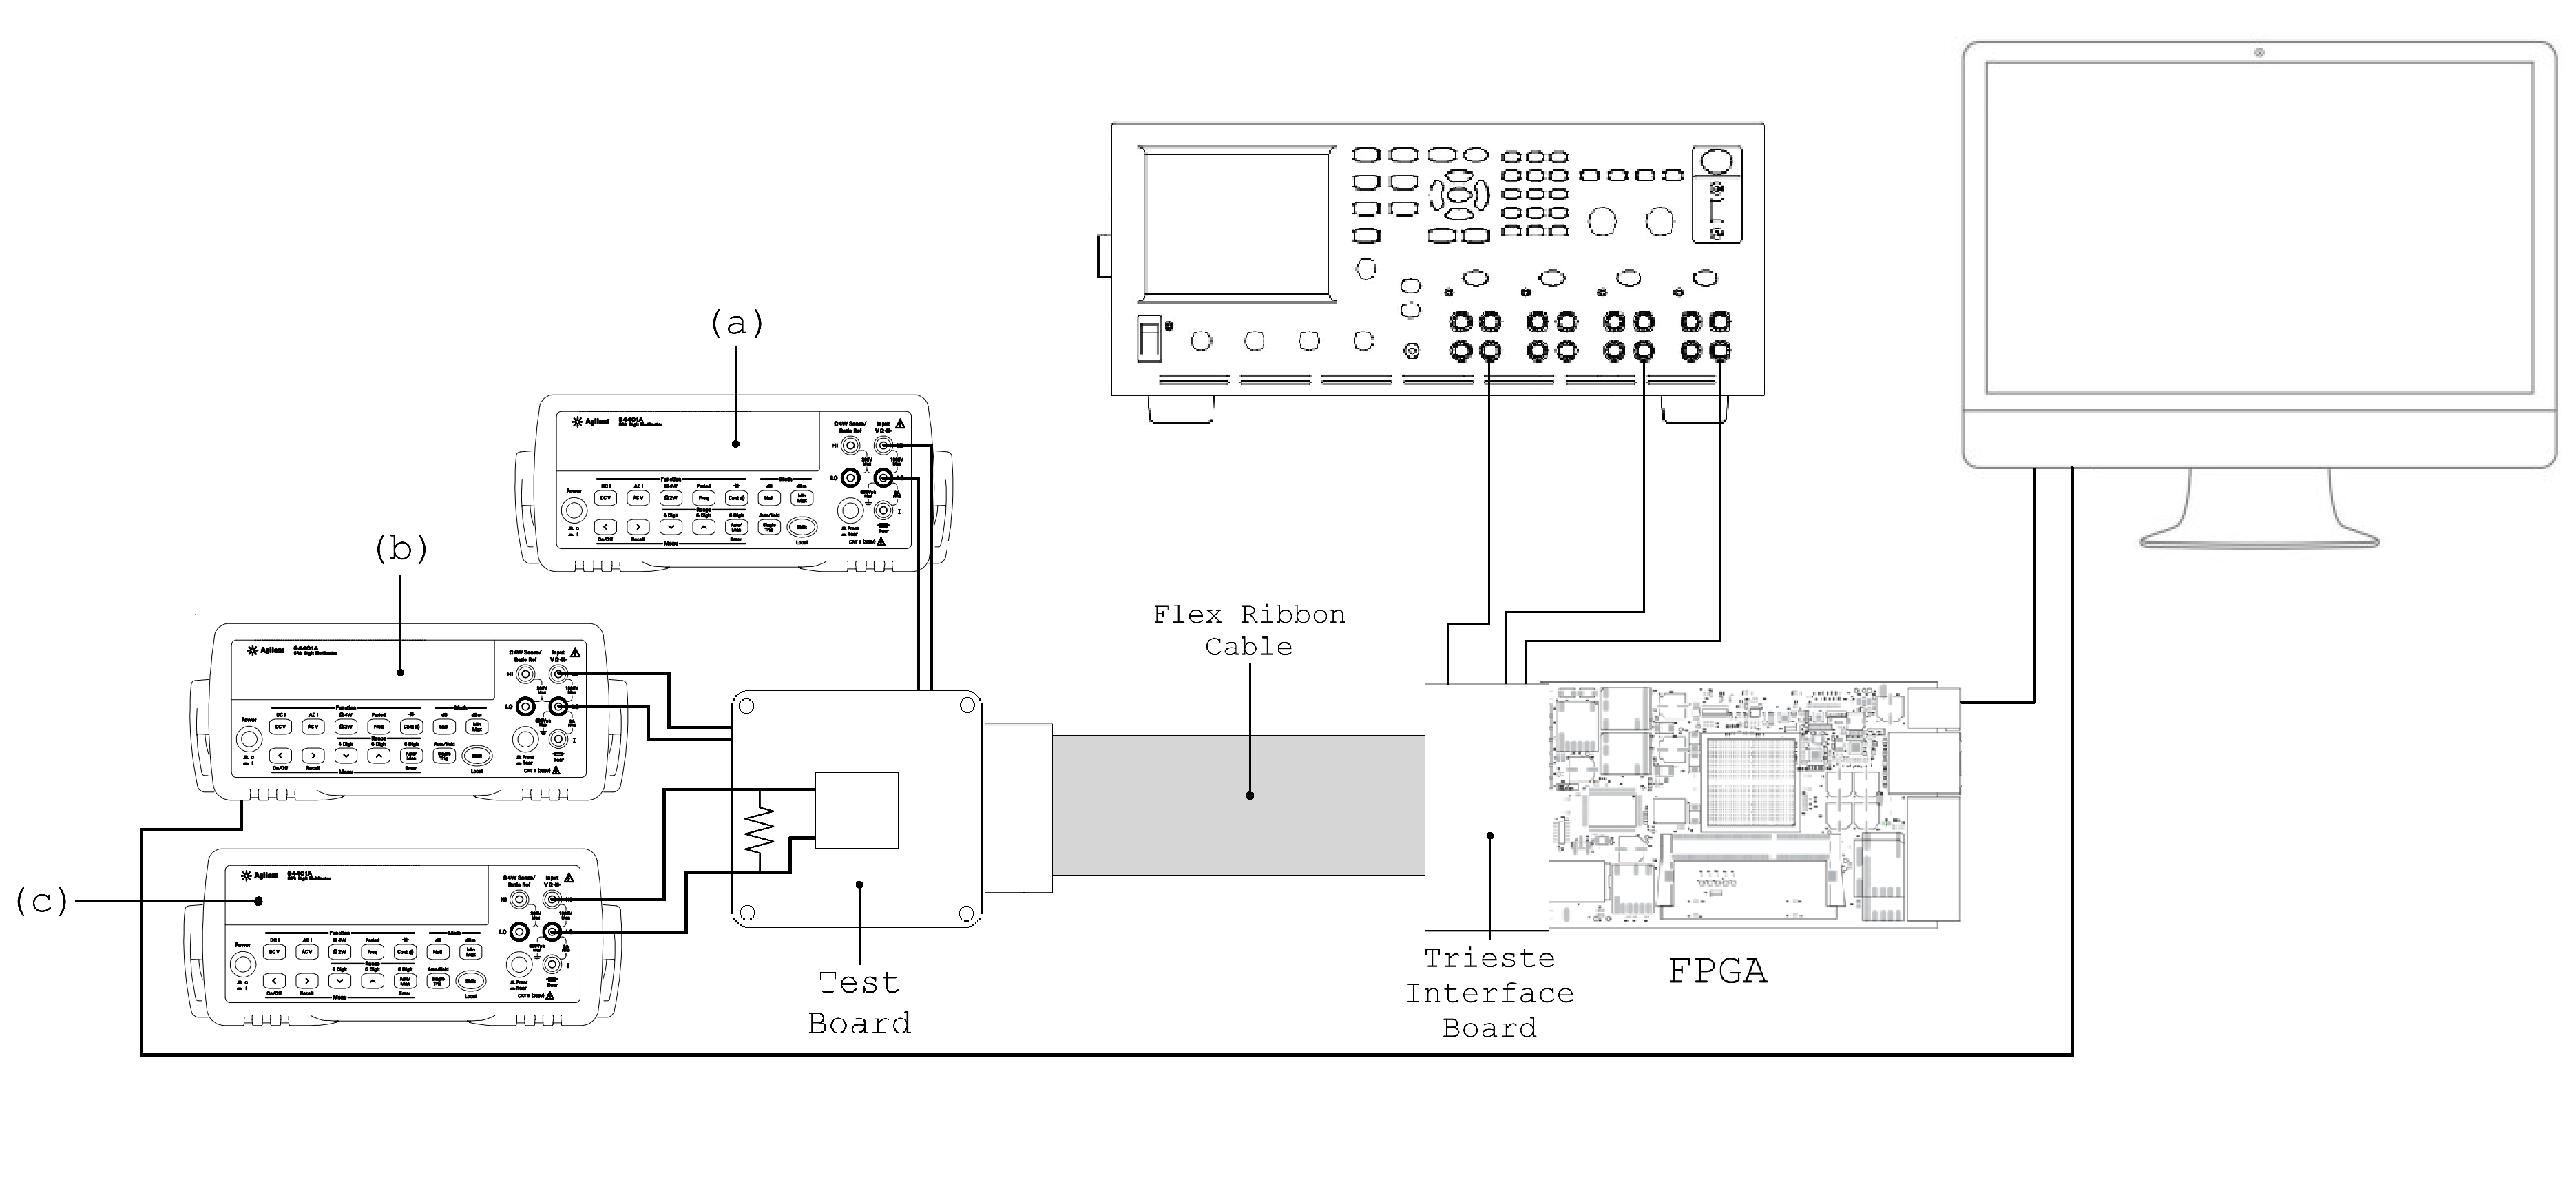
\includegraphics[width=1\textwidth]{Images/chap1/test_setup_test_board_csavrefgm_auto.png}
    \caption{SLIDER32 ASIC test board setup \texttt{1}.}
    \label{figTESTBOARDsetup1}
\end{figure}

\vspace{-1cm}

\begin{figure}[ht]
    \centering
    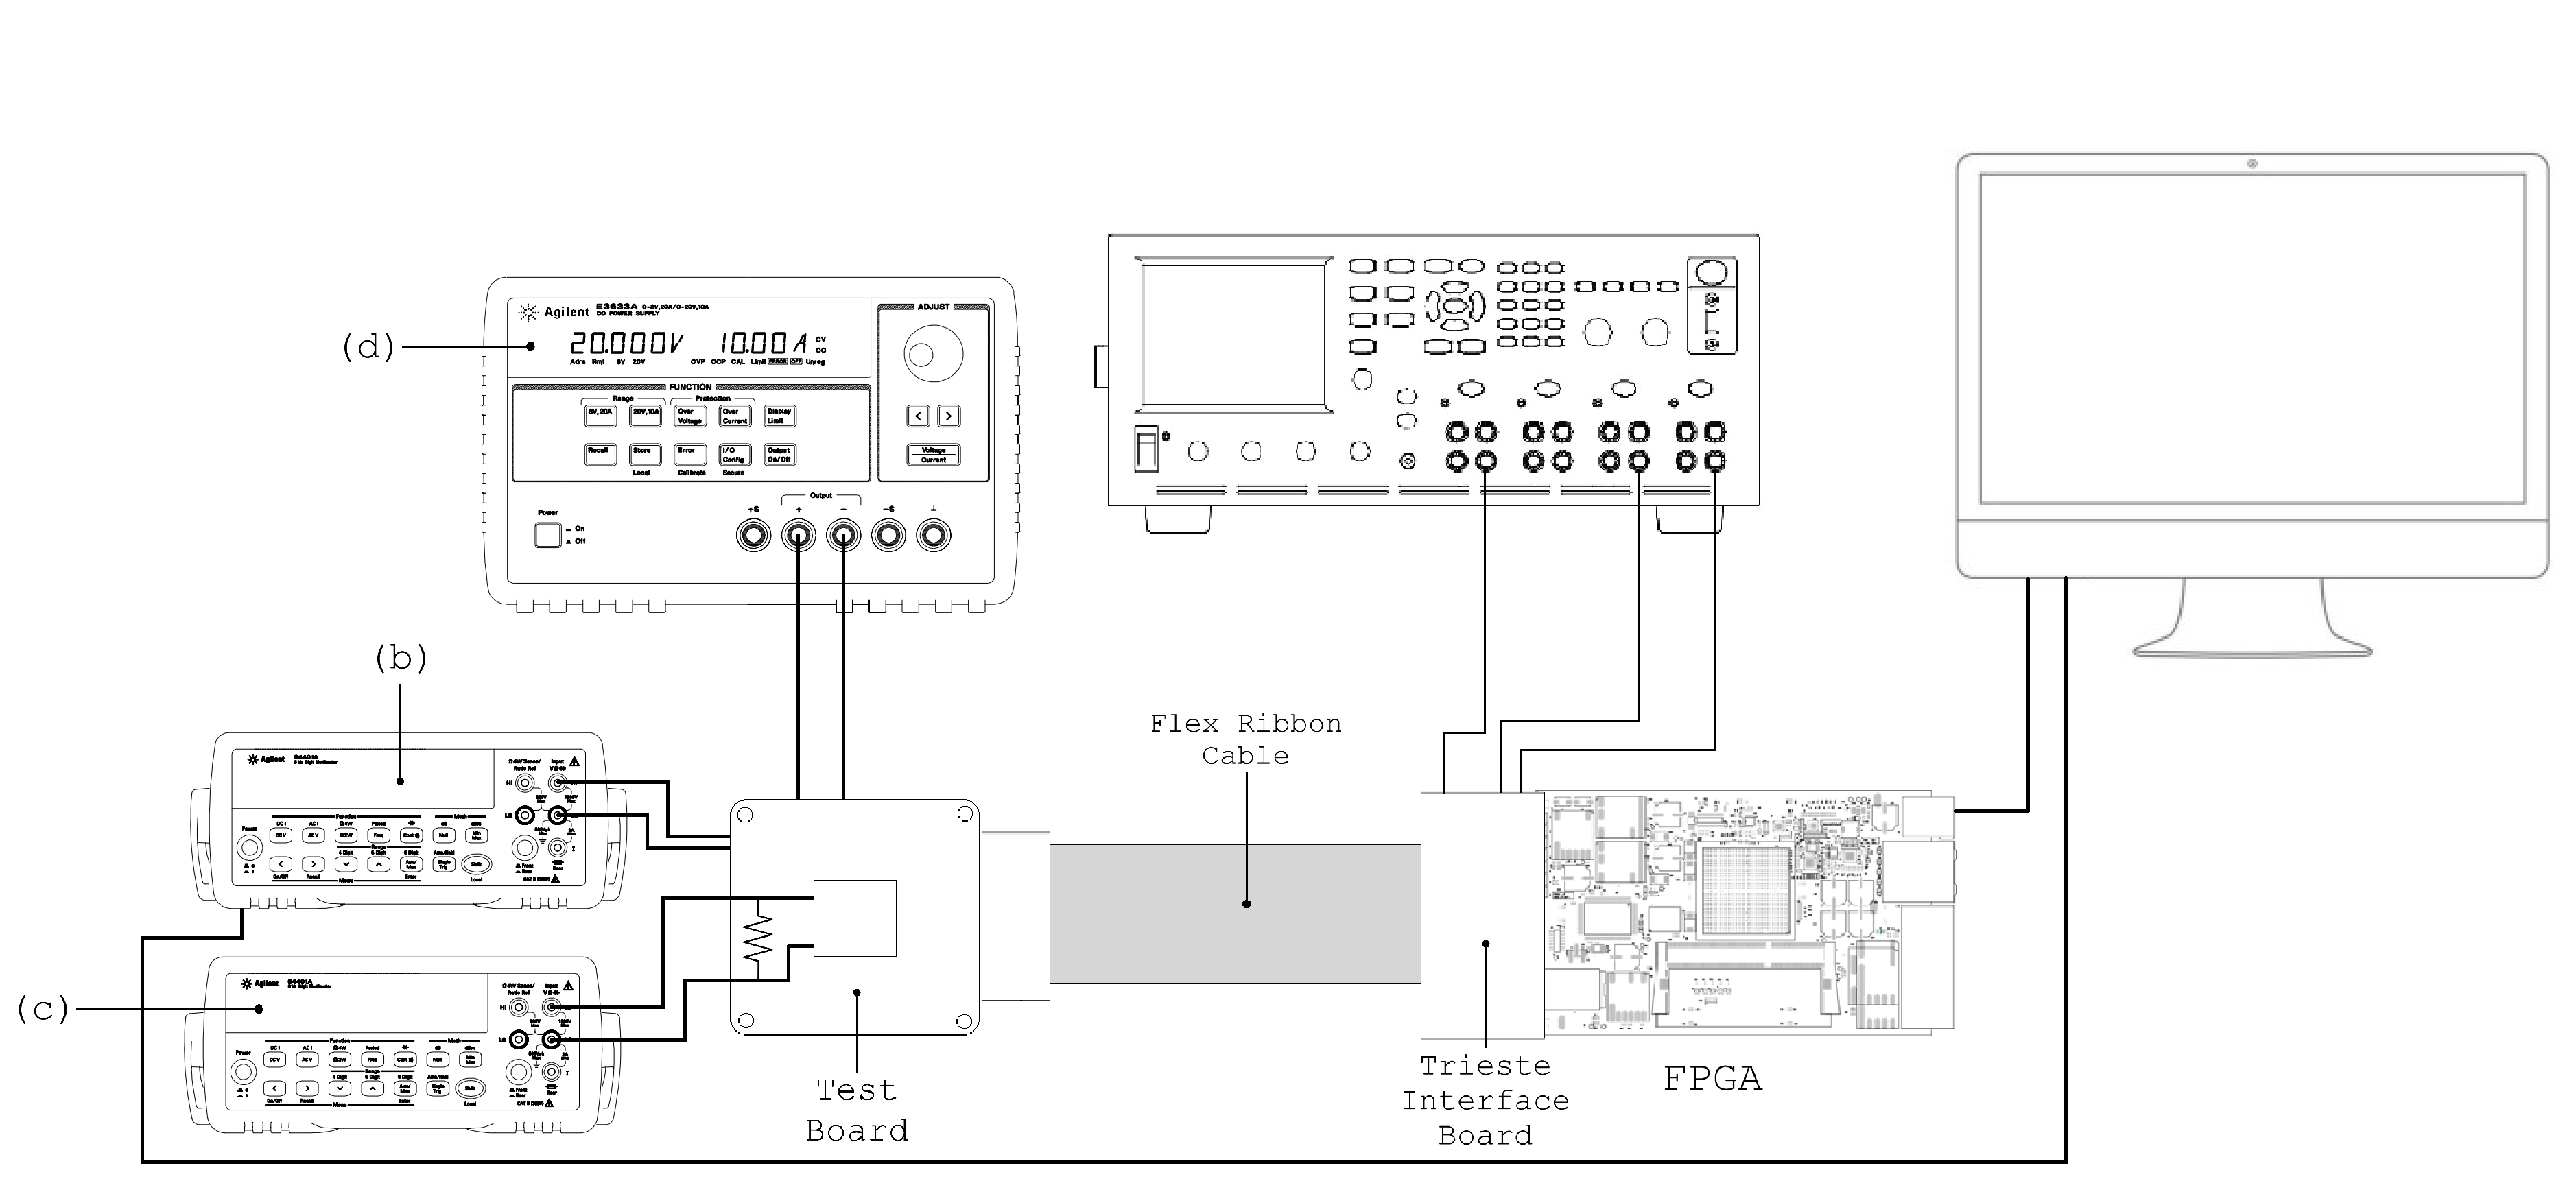
\includegraphics[width=1\textwidth]{Images/chap1/test_setup_test_board_csavrefgm_530mv.png}
    \caption{SLIDER32 ASIC test board setup \texttt{2}.}
    \label{figTESTBOARDsetup2}
\end{figure}

\par
\noindent
Both variants comprise the components discussed in the following.

\begin{itemize}
    \itemsep0em 
    \item A custom designed test board that allows tests to be performed on the ASIC without having to solder it to the board and then desolder it. This is made possible by a specific socket that allows the ASIC to be mounted and removed without having to solder it to the test board. This solution also allows several ASICs to be tested using a single board, although being not being the case of the proposed measurements, that involved only ASIC No. \texttt{536}.
    \item A Keysight N6705C DC Power analyser providing both analog and digital voltages to the test board. \hyperref[figKeysightFEBtb]{Figure \ref{figKeysightFEBtb}} shows a screen capture of the power supply. Specifically, channel \texttt{1} provides the analog supply voltage (\SI{2.4}{\volt}), channel \texttt{3} provides the digital supply voltage (\SI{2.4}{\volt}) and channel \texttt{4} the 16-bit calibration DAC supply voltage (\SI{3.6}{\volt}).
    
    \begin{minipage}{\linewidth}
    \vspace{0.4cm}
        \centering
        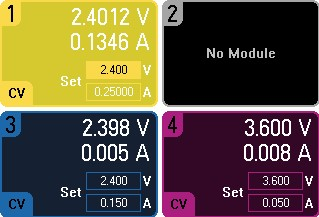
\includegraphics[width=0.5\textwidth]{Images/chap1/power_supply_screen_TB.jpg}
        \captionof{figure}{Keysight N6705C DC power analyser displayed voltages and currents on channels \texttt{1}, \texttt{3} and \texttt{4}.}
        \label{figKeysightFEBtb}
        \vspace{0.4cm}
    \end{minipage}
    
    \item An interface board specifically designed to route the power supplies and the signals trough the flex ribbon cable to the test board.
    \item A flex ribbon cable connecting the interface board to the main test board.
    \item An ALTERA Cyclone V Field Programmable Gate Array (FPGA).
    \item A PC running a Python-based testing program called \texttt{GAPS\_ModuleTester}, currently in its 4th version, connected to the FPGA via two Universal Serial Bus (USB) cables. This software has been specifically developed to perform a series of tests on the SLIDER32 ASIC and it is later described in \hyperref[sec21]{Section \ref{sec21}}.
    \item An Agilent 34401A digital multimeter \texttt{(b)} used to measure the global threshold voltage generated by an 8-bit DAC described in \hyperref[thresholdVoltageANALYSIS]{Section \ref{thresholdVoltageANALYSIS}}.
    \item An Agilent 34401A digital multimeter \texttt{(c)} used to measure the reference current as a voltage drop across a \SI{18}{\kilo\ohm} resistor mounted on the test board.
\end{itemize}

\par
Specific to version \texttt{1} of the test setup is the Agilent 34461A digital multimeter \texttt{(a)} that has been used to measure the \texttt{CSAVrefGM} voltage, automatically regulated by a bandgap with respect to the temperature at which the system operates in order to guarantee the correct gain of the readout channel.

\par
Version \texttt{2} of the test setup employs a Keysight E3631A DC power supply \texttt{(d)} in order to force the \texttt{CSAVrefGM} voltage to a fixed \SI{530}{\milli\volt} value. This voltage corresponds to the one provided by the bandgap at a temperature of \SI{-40}{\celsius}.

\par
The test board has been placed in a climate chamber (model ACS DY110) at temperatures spanning from \SI{-40}{\celsius} to \SI{30}{\celsius} with \SI{10}{\celsius} increments. The \SI{-40}{\celsius} to \SI{-30}{\celsius} region has been spanned with \SI{2}{\celsius} increments. In each test, before performing a test session, the climate chamber has been maintained at the desired temperature for 15 minutes in order to ensure that the electronics reached the correct temperature.

%-------------------------------------------------------------------------------
%	Current reference analysis
%-------------------------------------------------------------------------------

\section{Current reference}

The analog front-end channel designed for the readout of the Si(Li) detectors of the GAPS experiment is comprised of several blocks, as discussed in detail in \hyperref[secGAPSfrontend]{Appendix \ref{secGAPSfrontend}}. Each element of the channel requires one or more current references to be properly biased. These references should remain  constant regardless of external conditions like temperature, variations in the ASIC supply voltage and process parameter mismatch during fabrication. To comply with this requirement, a solution where the reference currents are generated starting from a precise Process, Voltage and Temperature (PVT) voltage reference has been adopted. Starting from this voltage, a 3-bit adjustable current can be obtained. This reference value has been chosen to be \SI{5}{\micro\ampere}.

\begin{figure}[h!]
    \centering
    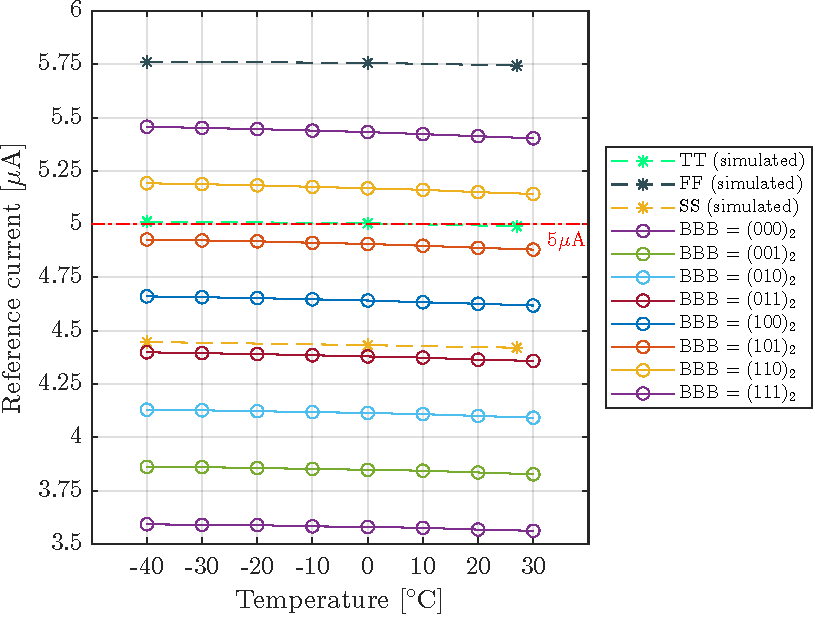
\includegraphics[width=0.7\textwidth]{Images/chap1/results/BGR_current/BGR_current_Xtemp_all-BBB.pdf}
    \caption{Reference current values for a given bias setting with respect to temperature varying from \SI{-40}{\celsius} to \SI{30}{\celsius} with \SI{10}{\celsius} increments.}
    \label{figBGRplotsXtempall}
\end{figure}

\par
A complete set of measurements of the reference current is shown in \hyperref[figBGRplotsXtempall]{Figure \ref{figBGRplotsXtempall}}. It has been taken by varying both the temperature from \SI{-40}{\celsius} to \SI{30}{\celsius} and the bias setting on all the $2^{3}$ possible values. It can be seen that, for a given bias setting expressed as a combination of 3 bits (\texttt{BBB}), the reference current remains almost constant with the temperature and experiences a variation that is presented in \hyperref[tableBGRvariation]{Table \ref{tableBGRvariation}}. The plot also shows the trend of the reference current as predicted by simulations in 3 different CMOS process corners, namely \textit{Typical-Typical} (TT), \textit{Fast-Fast} (FF) and \textit{Slow-Slow} (SS).

\par
The reference current has been evaluated by measuring the voltage drop across the resistor $R_{\textit{3}}$ on the test board, a 0603 SMD resistor with \SI{0.1}{\percent} tolerance and \SI{10}{ppm/\celsius} temperature coefficient. The current value has been calculated as

\begin{equation}
    I_{ref} = \frac{V_{ref}}{R_{\textit{3}}}
\end{equation}

It is possible to see that, among all bias settings (\texttt{BBB}), the one being the closest to the \SI{5}{\micro\ampere} reference value is \texttt{101} at almost every temperature considered, thus validating the choice of using this bias setting as the default one in all the other tests performed.

\begin{table}[h!]
    \centering
    \begin{tabular}{c c c c} 
        \Xhline{2\arrayrulewidth}
        \multicolumn{1}{p{2.6cm}}{\T \centering Bias setting $[\texttt{BBB}]$ } & 
        \multicolumn{1}{p{3.2cm}}{\centering Reference current \\ at \SI{-40}{\celsius} $[\SI{}{\milli\ampere}]$} &
        \multicolumn{1}{p{3.2cm}}{\centering Reference current \\ at \SI{30}{\celsius} $[\SI{}{\milli\ampere}]$} & 
        \multicolumn{1}{p{1.8cm}}{\centering Variation \\ $[\%]$ \B} \\
        \hline
        000 & 3.59 & 3.56 & 0.85 \T\B \\
        001 & 3.86 & 3.83 & 0.90 \T\B \\
        010 & 4.13 & 4.09 & 0.91 \T\B \\
        011 & 4.40 & 4.36 & 0.92 \T\B \\
        100 & 4.66 & 4.62 & 0.92 \T\B \\
        101 & 4.93 & 4.88 & 0.96 \T\B \\
        110 & 5.19 & 5.14 & 0.96 \T\B \\
        111 & 5.46 & 5.40 & 0.99 \T\B \\
        \Xhline{2\arrayrulewidth}
    \end{tabular}
    \caption{Reference current values and variations with respect to temperature from \SI{-40}{\celsius} to \SI{30}{\celsius} for each bias settings.}
    \label{tableBGRvariation}
\end{table}

\par
\hyperref[figBGRplotXbias]{Figure \ref{figBGRplotXbias}} proposes on the left the plot of the reference current at temperatures varying from \SI{-40}{\celsius} to \SI{30}{\celsius} with respect to the bias setting. On the right, the measurement at \SI{30}{\celsius} is compared with simulations and a previously taken measurement at a temperature of \SI{27}{\celsius}.

\begin{figure}[h!]
    \centering
    \begin{tabular}{cc}
        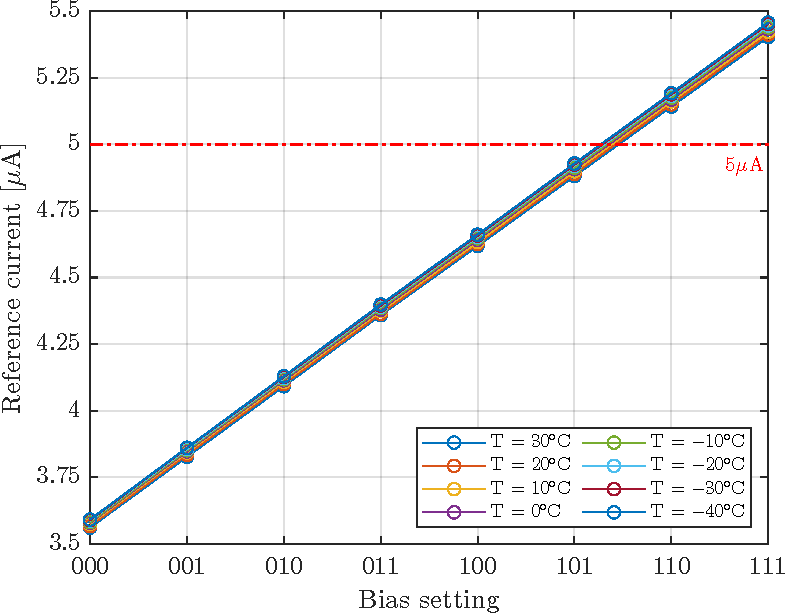
\includegraphics[width=0.475\textwidth]{Images/chap1/results/BGR_current/BGR_current_XBBB.pdf} & 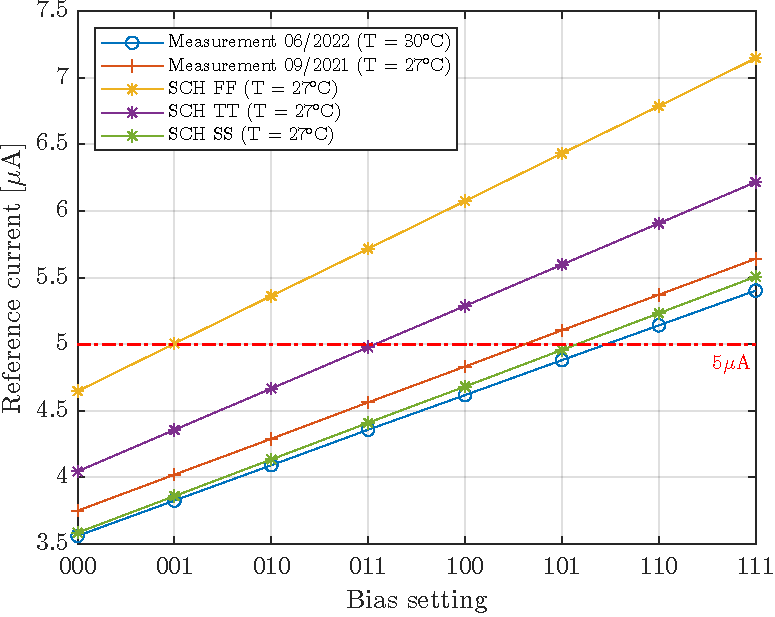
\includegraphics[width=0.475\textwidth]{Images/chap1/results/BGR_current/BGR_current_XBBB_27C_sim.pdf}\\
    \end{tabular}
    \caption{Current reference values given temperature with respect to bias setting (on the left) and with respect to simulations at \SI{27}{\celsius} (on the right).}
    \label{figBGRplotXbias}
\end{figure}

\par
\hyperref[figBGRplotsnormalised]{Figure \ref{figBGRplotsnormalised}} reports the normalised reference current measured at temperatures varying from \SI{-40}{\celsius} to \SI{30}{\celsius} and compared to the values coming from simulations in the same temperature range.

\begin{figure}[h!]
    \centering
    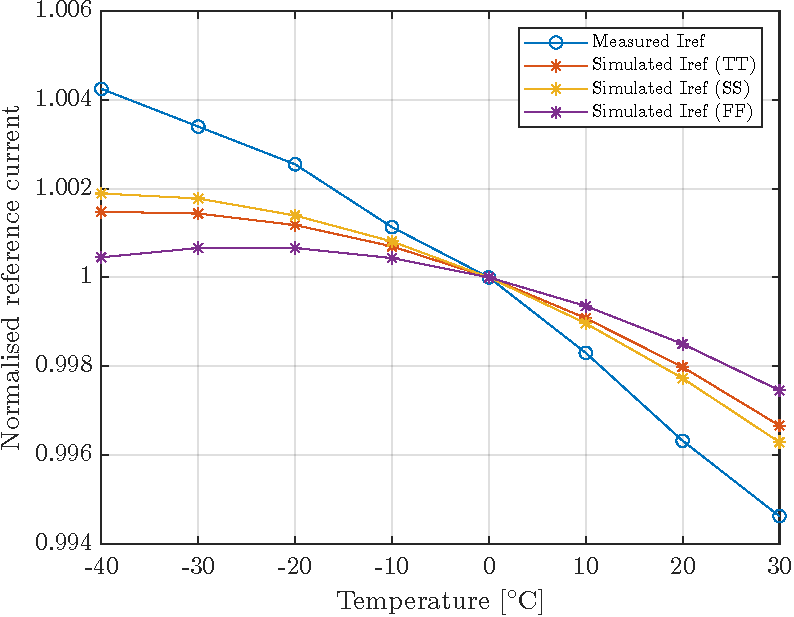
\includegraphics[width=0.7\textwidth]{Images/chap1/results/BGR_current/BGR_current_normal_Iref.pdf}
    \caption{Normalised current reference values compared to TT, FF and SS simulations with respect to temperature from \SI{-40}{\celsius} to \SI{30}{\celsius}.}
    \label{figBGRplotsnormalised}
\end{figure}

\par
The reference current measurements have also been evaluated by extracting the temperature coefficient, $\alpha$. The temperature coefficient can be defined as the ratio of change in resistance with respect to a variation of one degree in temperature and can be expressed as

\begin{equation}
    \alpha = \frac{1}{I_{T_{0}}} \cdot \frac{\Delta I}{\Delta T}
\end{equation}

\noindent
where $I_{T_{0}}$ represents the current value measured at a reference temperature of \SI{0}{\celsius} and $\Delta T$ is defined as the difference between the maximum and the minimum temperatures at which the measurements have been performed and it can be expressed as

\begin{equation}
    \Delta T = \lvert T_{max} - T_{min} \rvert
\end{equation}

\noindent
In the same way, $\Delta I$ represents the difference between the current measured at the minimum temperature, $T_{min}$, and that measured at the maximum temperature, $T_{max}$, and is defined as 

\begin{equation}
    \Delta I = I_{T_{min}}- I_{T_{max}}
\end{equation}

\noindent
In the specific case of the presented measurements and simulations, the temperature delta is equal to $\Delta T = \SI{70}{\celsius}$. The estimated temperature coefficients, expressed as \SI{}{ppm/\celsius}, are reported in \hyperref[tabtempcoefficients]{Table \ref{tabtempcoefficients}}. It is clear to see that the temperature coefficient of the measured reference current is above every one of the temperature coefficients evaluated over the readings coming from simulations in all of the 3 process corners. %This behaviour can be associated to [?].

\begin{table}[ht]
    \centering
    \begin{tabular}{c c} 
        \Xhline{2\arrayrulewidth}
        & $\alpha$ [\SI{}{ppm/\celsius}] \T\B \\
        \hline
        Measured & 137.42 \T\B \\
        TT model & 68.57 \T\B \\
        SS model & 80.00 \T\B \\
        FF model & 42.86 \T\B \\
        \Xhline{2\arrayrulewidth}
    \end{tabular}
    \caption{Estimated temperature coefficients.}
    \label{tabtempcoefficients}
\end{table}


%-------------------------------------------------------------------------------
%	Input-output channel trans-characteristic
%-------------------------------------------------------------------------------

\section{Input-output channel trans-characteristic}
\label{testboardFDT}

In this Section a description of the temperature effects on the channel input-output characteristic is given. The curve trend is due to the Charge Sensitive Amplifier (CSA) circuit block, which is responsible for converting the incident charge on the Si(Li) detector into a voltage signal that is subsequently supplied to the shaper, described in \hyperref[shaper]{Section \ref{shaper}}. 

\par
The CSA is based on an inverting gain stage and a feedback capacitor where charge restoration is achieved by a continuous-time Krummenacher network \cite{krummenacher_1991_pixel}. The main feature of the CSA is the dynamic signal compression that is achieved by implementing the feedback capacitor with an NMOSFET operating in the inversion mode \cite{manghisoni_2018_dynamic}. In this transistor, source and drain are shorted to form the capacitor terminal connected to the amplifier input, while the gate terminal is connected to the output. At small signal amplitudes, the gate-to-channel voltage is smaller than the transistor threshold voltage and the capacitance is equal to the sum of gate-source and gate-drain overlap capacitances. At larger signal amplitudes, the gate-to-channel voltage becomes larger than the the transistor threshold and the capacitance increases including also the gate-to-channel capacitance. According to this mechanism, the feedback capacitance increases from \SI{175}{\femto\farad} at small input signal amplitudes to \SI{14.7}{\pico\farad} at large signal amplitudes. \hyperref[figCSAschematic]{Figure \ref{figCSAschematic}} shows the schematic of the CSA, with the nonlinear MOSFET feedback capacitance.

\begin{figure}[h!]
    \centering
    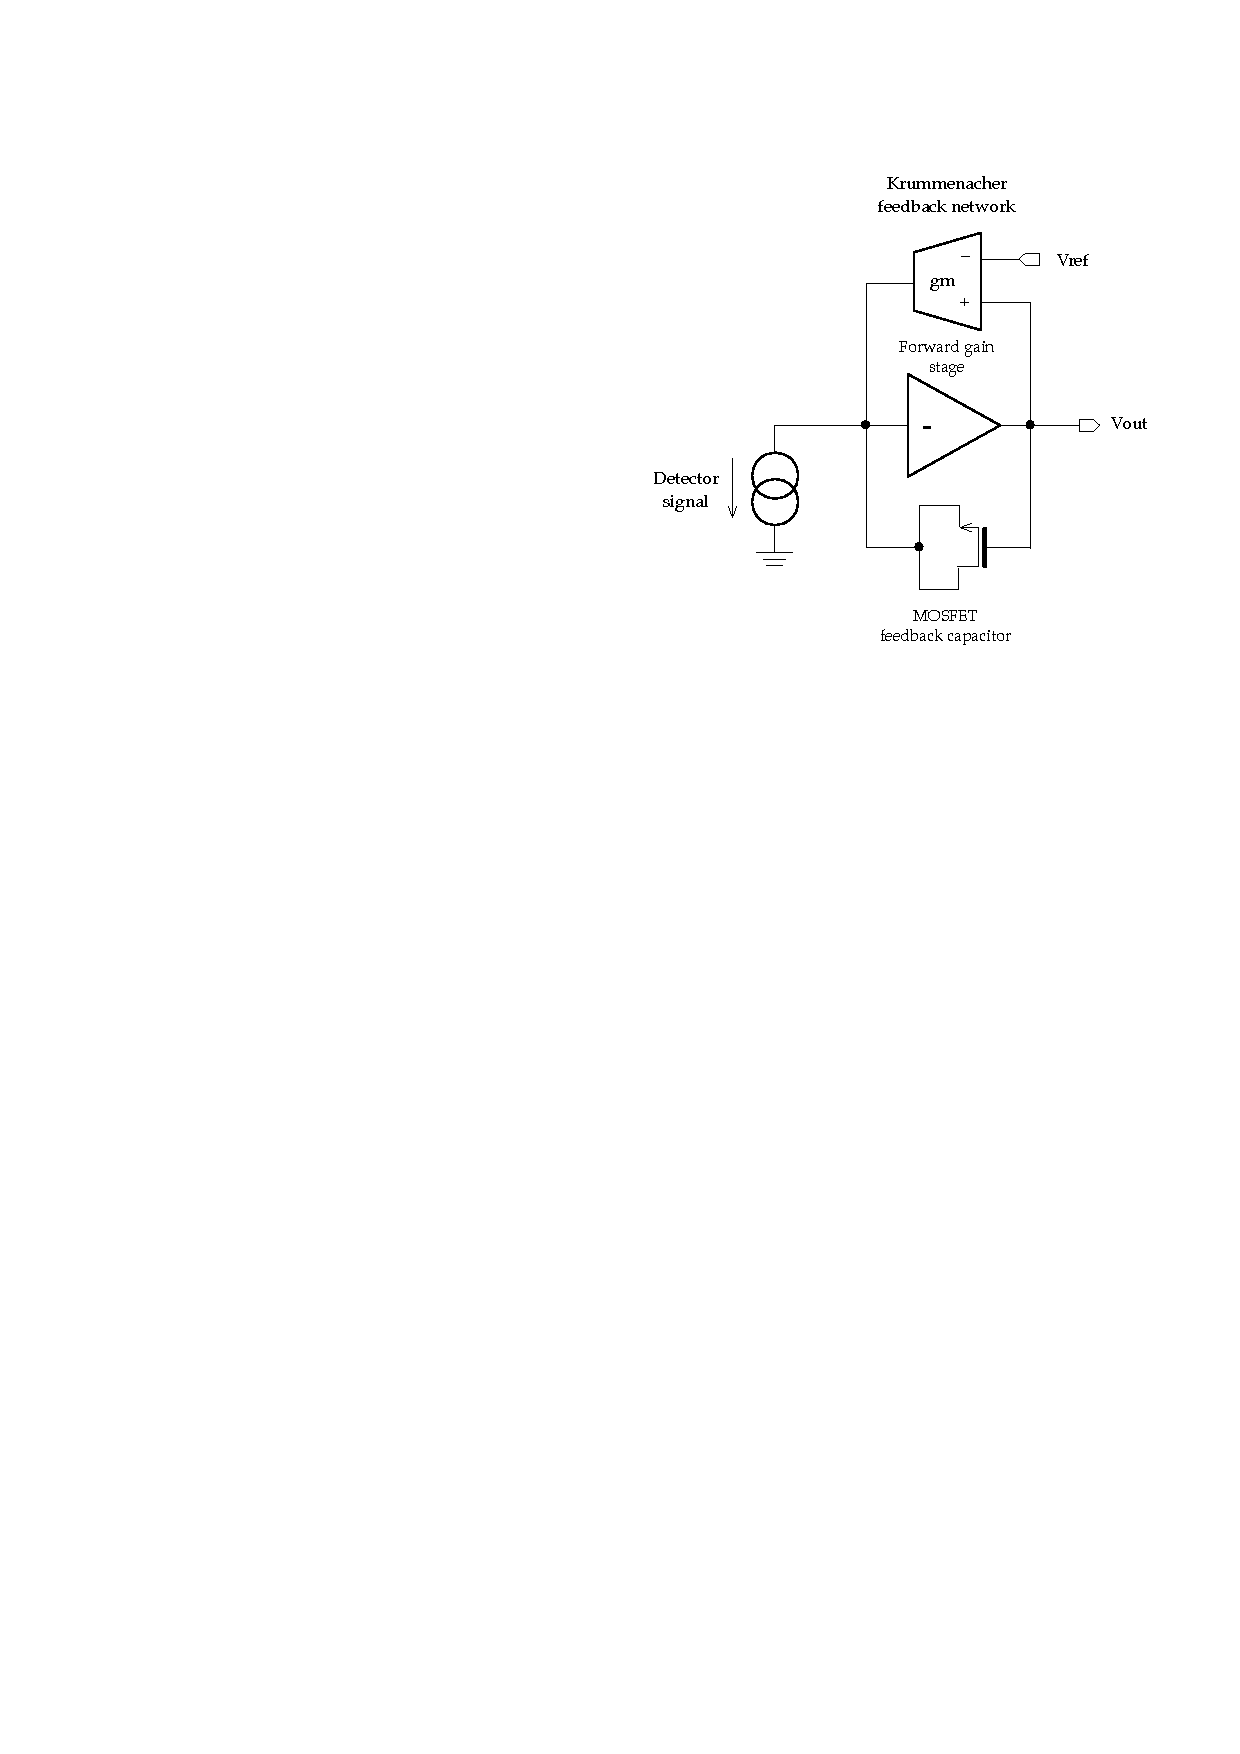
\includegraphics[width=0.65\textwidth]{Images/chap1/CSA_schematic.pdf}
    \caption{Schematic of the charge-sensitive preamplifier, with the forward gain stage, the nonlinear MOSFET capacitor and the Krummenacher feedback network.}
    \label{figCSAschematic}
\end{figure}

\par
A reference voltage in the Krummenacher feedback network, denoted as $V_{ref}$ in \hyperref[figCSAschematic]{Figure \ref{figCSAschematic}} and referred to as \texttt{CSAVrefGM} in the following, makes it possible to adjust the amplifier output voltage, so that the signal amplitude at which the CSA switches from high to low gain can be finely tuned, compensating for process and temperature variations. In the nominal setting, the kink in the input-output characteristic occurs at an energy deposited on the detector of about \SI{1}{\mega\electronvolt}.

\par
In order to obtain the input-output characteristic of the CSA, the channel output must be sampled precisely at the peaking time, set by bit configuration \texttt{TTT}, that for the presented measurements has been chosen to be $\tau_{p} = \SI{0.98}{\micro\second}$ (peaking time 4, meaning \texttt{TTT} equal to \texttt{100}). The value of the injected charge ranges from 0 to \SI{60000}{DACu} (DAC unit) and it can be converted in the equivalent energy value using the conversion factor of \SI{1}{DACu} = \SI{0.841}{\kilo\electronvolt}, whose value is later derived in \hyperref[eqConversionFactor]{Equation \ref{eqConversionFactor}}, therefore the range can be equivalently expressed as spanning from 0 to \SI{50.46}{\mega\electronvolt}.

\par
\hyperref[figFDTplotauto0011]{Figure \ref{figFDTplotauto0011}} shows the input-output trans-characteristic obtained as the mean of the 32 channels of the ASIC with respect to temperature ranging from \SI{-40}{\celsius} to \SI{30}{\celsius}. In this case, the \texttt{CSAVrefGM} voltage has been left free to automatically adapt to the given temperature and has been measured using the test setup \texttt{1} described in \hyperref[figTESTBOARDsetup1]{Figure \ref{figTESTBOARDsetup1}}. The CSA REFERENCE REGULATION setting (\texttt{HRRR} bits) has been set to \texttt{0011}.

\begin{figure}[h!]
    \centering
    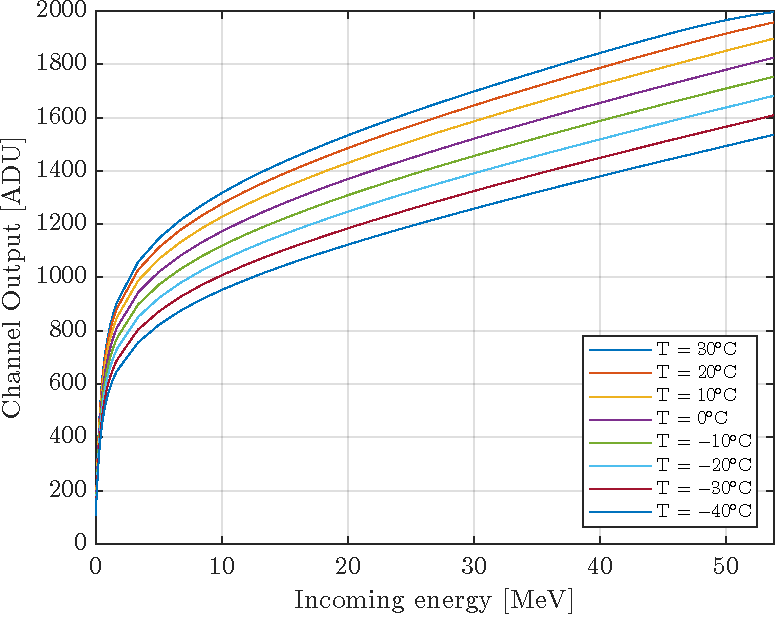
\includegraphics[width=0.68\textwidth]{Images/chap1/results/FDT/fdt_csavrefgm_auto_tau6_keV_0011.pdf}
    \caption{Mean input-output channel trans-characteristics with respect to temperature varying from \SI{-40}{\celsius} to \SI{30}{\celsius} and automatically regulated \texttt{CSAVrefGM} voltage.}
    \label{figFDTplotauto0011}
\end{figure}

The first bit, \texttt{H}, is set to \texttt{0} when the ASIC is operated at \SI{-40}{\celsius} and to \texttt{1} when operated at room temperature. The last three bits, \texttt{RRR}, allow to set the charge sensitive amplifier reference.

\noindent
The \texttt{CSAVrefGM} values measured at each temperature are presented in \hyperref[tablecsavref]{Table \ref{tablecsavref}}. It comprises measurements taken with \texttt{HRRR} respectively set to \texttt{0011} and \texttt{0111} and the relative percentage variation between the two. It is of immediate comprehension that neither configuration is capable of reaching the desired \SI{530}{\milli\volt} at \SI{-40}{\celsius}. It is in fact necessary to set \texttt{RRR} to \texttt{111} in order to get the closest possible to the reference value.

\begin{table}[ht]
    \centering
    \begin{tabular}{c c c c} 
        \Xhline{2\arrayrulewidth}
        \multirow{2}{*}{Temperature [\SI{}{\celsius}]} \T & \multicolumn{2}{p{5cm}}{\centering \texttt{CSAVrefGM} $[\SI{}{\milli\volt}]$} \T & \multirow{2}{*}{Variation [\SI{}{\percent}]} \\
        \cline{2-3}
        & \texttt{HRRR = 0011} & \texttt{HRRR = 0111} \B\\
        \hline
        30 & 360.5 & 370.9 & 2.80 \T\B \\
        20 & 383.1 & 392.0 & 2.27 \T\B \\
        10 & 405.3 & 413.8 & 2.05 \T\B \\
        0 & 432.1 & 436.3 & 6.73 \T\B \\
        -10 & 450.5 & 458.4 & 1.72 \T\B \\
        -20 & 473.2 & 480.6 & 1.54 \T\B \\
        -30 & 495.1 & 504.3 & 1.82 \T\B \\
        -40 & 517.5 & 525.8 & 1.58 \T\B \\
        \Xhline{2\arrayrulewidth}
    \end{tabular}
    \caption{\texttt{CSAVrefGM} voltage measured at temperatures varying from \SI{-40}{\celsius} to \SI{30}{\celsius} with CSA REFERENCE REGULATION bits set to \texttt{0011} and \texttt{0111} respectively.}
    \label{tablecsavref}
\end{table}

\hyperref[figFDTplot530mV]{Figure \ref{figFDTplot530mV}} shows the mean input-output channel trans-characteristics calculated over the 32 channels of the ASIC given temperatures ranging from \SI{-40}{\celsius} to \SI{30}{\celsius}. In this case, the \texttt{CSAVrefGM} has been set to a fixed value of \SI{530}{\milli\volt} using the test setup \texttt{2} described in \hyperref[figTESTBOARDsetup2]{Figure \ref{figTESTBOARDsetup2}}. It is possible to notice that by fixing the voltage to the automatically regulated value at \SI{-40}{\celsius} regardless of the temperature, the channel transfer function assumes an unwanted trend.  

\begin{figure}[h!]
    \centering
    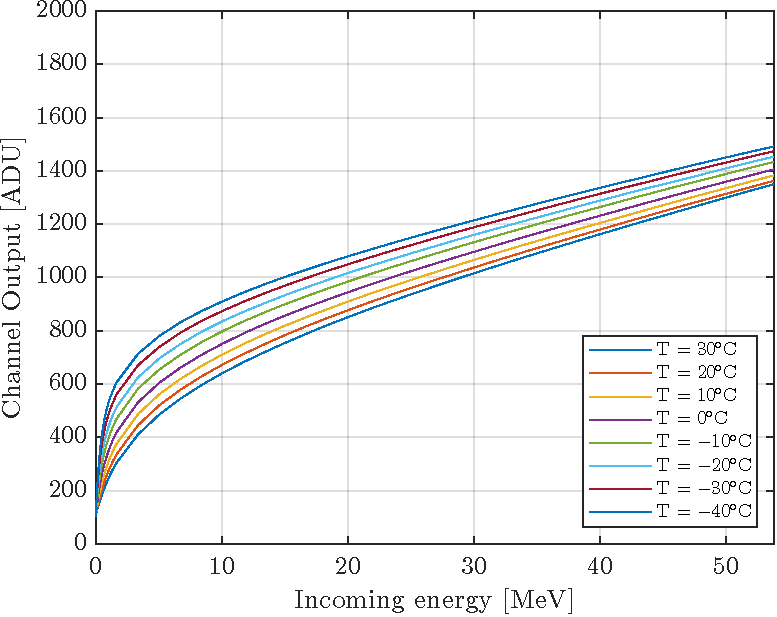
\includegraphics[width=0.68\textwidth]{Images/chap1/results/FDT/fdt_csavrefgm_530mV_tau6_keV.pdf}
    \caption{Mean input-output channel trans-characteristics given temperatures varying from \SI{-40}{\celsius} to \SI{30}{\celsius} and \texttt{CSAVrefGM} voltage fixed to \SI{530}{\milli\volt}.}
    \label{figFDTplot530mV}
\end{figure}

\par
As it can be seen from the charts, the channel input-output trans-characteristic is a non-linear function that can be described as an almost piecewise linear function whose sensitivity is determined by the dynamic compression feature of the CSA. Through this non-linearity the resolution of the signals changes as a function of the charge generated by the energy release of the incident particle in the detector: in a low energy range, the resolution of the signal must be high and, consequently, the charge signal must be amplified adequately and vice versa in the high energy range. This implies that in the first segment the transfer function has a high slope. In the high energy range, however, the required resolution is not so stringent, consequently the gain of the transfer function is less than that in the first section. The channel transfer function can therefore be divided into two regions, based on the incoming energy:

\begin{itemize}
    \itemsep0em
    \item \textit{Low energy region}: Also known as X-ray detection region, it ranges from approximately 10 to \SI{100}{\kilo\electronvolt}.
    \item \textit{High energy region}: Also described as muon detection region, it spans an energy range comprised between 40 and \SI{55}{\mega\electronvolt}.
\end{itemize}

\noindent
In both X-ray and muon detection regions, the characteristic exhibits a linear behaviour and can be expressed as

\begin{equation}
    y = p + g \cdot x
    \label{FDTlinearModel}
\end{equation}

\noindent
where

\begin{itemize}
    \itemsep0em
    \item \textbf{y} [\SI{}{ADU}] (Analog Digital Unit) is the channel output.
    \item \textbf{p} [\SI{}{ADU}] is the pedestal, which consists of a repeated sampling of the channel output without charge injected.
    \item \textbf{g} [\SI{}{ADU/\kilo\electronvolt}] is the channel gain.
    \item \textbf{x} [\SI{}{\kilo\electronvolt}] is the input energy.
\end{itemize}

The effect of temperature variation on the channel transfer function has been studied by evaluating gain and pedestal in both X-ray and muon detection regions. For each of the two parameters, a linear regression model has been defined in order to study the trend on both gain and pedestal with respect to temperature ranging from \SI{-40}{\celsius} to \SI{30}{\celsius}, which has been demonstrated to have an almost perfect linear trend. For the gain analysis, the following linear regression model has been defined.

\begin{equation}
    g = g_{\textit{0}} + g_{\textit{1}} \cdot (T - T_{\textit{0}})
    \label{equationGain}
\end{equation}

\noindent
The intercept $g_{\textit{0}}$ is measured in \SI{}{ADU/\kilo\electronvolt}, the slope $g_{\textit{1}}$ in ADU \SI{}{\kilo\electronvolt^{-1}} \SI{}{\celsius^{-1}} and the reference temperature has been set to $T_{\textit{0}} = \SI{0}{\celsius}$. For the study of the gain in the high-energy region, $g_{0}$ is reported in \SI{}{ADU/\mega\electronvolt}, while $g_{1}$ is expressed in ADU \SI{}{\mega\electronvolt^{-1}} \SI{}{\celsius^{-1}}. Similarly, the following linear regression model has been defined for pedestal analysis.

\begin{equation}
    p = p_{\textit{0}} + p_{\textit{1}} \cdot (T - T_{\textit{0}})
\end{equation}

\noindent
The intercept $p_{\textit{0}}$ is measured in \SI{}{ADU}, the slope $p_{\textit{1}}$ in \SI{}{ADU/\celsius} and the reference temperature has been set to $T_{\textit{0}} = \SI{0}{\celsius}$. 

\par
\hyperref[tableFDTgainpedestal1]{Table \ref{tableFDTgainpedestal1}} provides the linear regression model coefficients for both gain and pedestal obtained upon the mean channel input-output characteristics measured at temperatures ranging between \SI{-40}{\celsius} and \SI{30}{\celsius}.

\begin{table}[ht]
    \centering
    \def\arraystretch{1.1}
    \begin{tabular}{c c c c c c c} 
        \Xhline{2\arrayrulewidth}
        & \multicolumn{3}{c}{Gain} & \multicolumn{3}{c}{Pedestal} \T\B \\
        \hline
        & $g_{\textit{0}}$ & $g_{\textit{1}}$ & R$^{2}$ & $p_{\textit{0}}$ & $p_{\textit{1}}$ & R$^{2}$ \T\B \\
        \hline
        \multicolumn{1}{p{4.5cm}}{\centering X-ray detection region \T \\ (10$\div$\SI{100}{\kilo\electronvolt})} & \multirow{2}{*}{1.25} & \multirow{2}{*}{0.006} & \multirow{2}{*}{0.997} & \multirow{2}{*}{182.32} & \multirow{2}{*}{0.651} & \multirow{2}{*}{0.985} \\
        \multicolumn{1}{p{4.5cm}}{\centering Muon detection region \B \\ (40$\div$\SI{55}{\mega\electronvolt})} & \multirow{2}{*}{12.27} & \multirow{2}{*}{0.024} & \multirow{2}{*}{0.989} & \multirow{2}{*}{1738} & \multirow{2}{*}{6.778} & \multirow{2}{*}{0.999} \T\B \\
        \Xhline{2\arrayrulewidth}
    \end{tabular}
    \caption{Gain and pedestal linear regression models coefficients obtained from measurements with automatically generated \texttt{CSAVrefGM} voltage and \texttt{HRRR} set to \texttt{0011}.}
    \label{tableFDTgainpedestal1}
\end{table}

\noindent
The channel peaking time has been set to $\tau_{p} = \SI{0.98}{\micro\second}$ (peaking time 4, \texttt{TTT} set to \texttt{100}), with \texttt{CSAVrefGM} voltage automatically generated and \texttt{HRRR} set to \texttt{0011}.

\par
\hyperref[tableFDTgainpedestal530]{Table \ref{tableFDTgainpedestal530}} presents the same linear regression models coefficients but in the case of fixed \texttt{CSAVrefGM} voltage, that has been set to \SI{530}{\milli\volt}.

\begin{table}[ht]
    \centering
    \begin{tabular}{c c c c c c c} 
        \Xhline{2\arrayrulewidth}
        & \multicolumn{3}{c}{Gain} & \multicolumn{3}{c}{Pedestal} \T\B \\
        \cline{1-7}
        & $g_{\textit{0}}$ & $g_{\textit{1}}$ & R$^{2}$ & $p_{\textit{0}}$ & $p_{\textit{1}}$ & R$^{2}$ \T\B \\
        \hline
        \multicolumn{1}{p{4.5cm}}{\centering X-ray detection region \T \\ (10$\div$\SI{100}{\kilo\electronvolt})} & \multirow{2}{*}{0.46} & \multirow{2}{*}{-0.012} & \multirow{2}{*}{0.992} & \multirow{2}{*}{128.66} & \multirow{2}{*}{-0.530} & \multirow{2}{*}{0.974} \T\B \\
        \multicolumn{1}{p{4.5cm}}{\centering Muon detection region \\ (40$\div$\SI{55}{\mega\electronvolt}) \B} & \multirow{2}{*}{12.61} & \multirow{2}{*}{0.033} & \multirow{2}{*}{0.997} & \multirow{2}{*}{1325.4} & \multirow{2}{*}{-2.406} & \multirow{2}{*}{0.988} \T\B \\
        \Xhline{2\arrayrulewidth}
    \end{tabular}
    \caption{Gain and pedestal linear regression models coefficients obtained from measurements with \texttt{CSAVrefGM} voltage set at a fixed value of \SI{530}{\milli\volt}.}
    \label{tableFDTgainpedestal530}
\end{table}

Graphs presented below show the trend of gain and pedestal with respect to temperature in the low and high energy regions for the configurations where \texttt{CSAVrefGM} is automatically adjusted (with \texttt{HRRR} set to \texttt{0011}) and set to \SI{530}{\milli\volt} respectively. The measurements were carried out by varying the temperature from \SI{-40}{\celsius} to \SI{30}{\celsius} in steps of \SI{10}{\celsius}, while the region between \SI{-40}{\celsius} and \SI{-30}{\celsius} was studied with steps of \SI{2}{\celsius}. 

% low energy gain
\begin{figure}[h!]
    \centering
    \begin{tabular}{cc}
        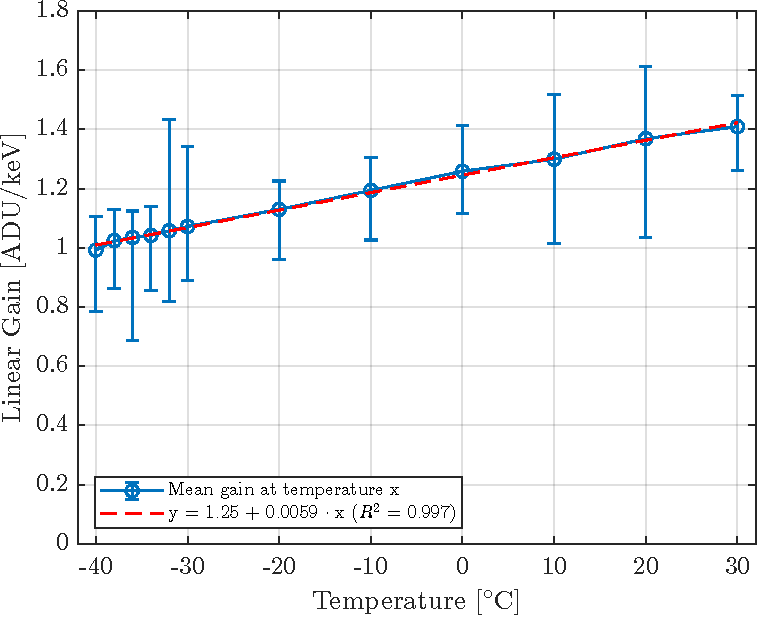
\includegraphics[width=0.475\textwidth]{Images/chap1/results/gain_pedestal/low_energy_gain_auto_0011.pdf} & 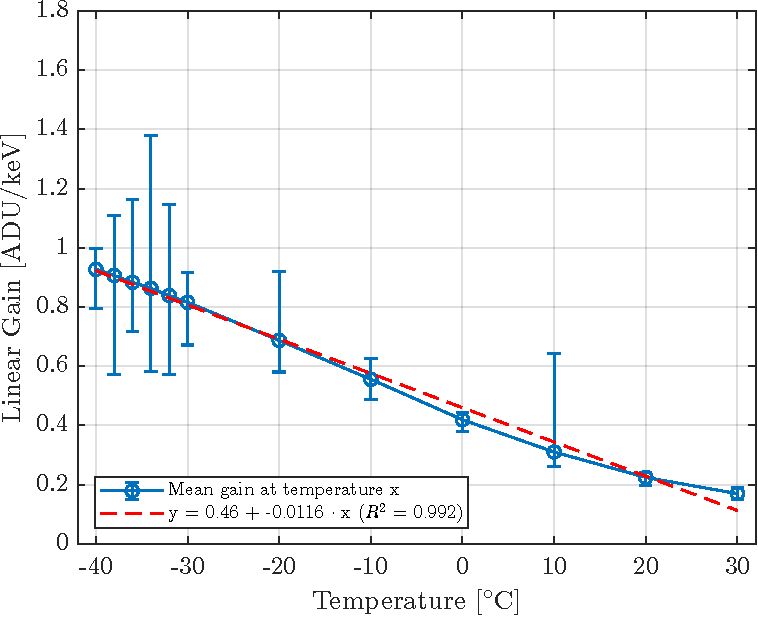
\includegraphics[width=0.475\textwidth]{Images/chap1/results/gain_pedestal/low_energy_gain_530mV.pdf}\\
    \end{tabular}
    \caption{Low energy gain trend with respect to temperature from \SI{-40}{\celsius} to \SI{30}{\celsius} for automatically regulated \texttt{CSAVrefGM} voltage (on the left) and fixed to \SI{530}{\milli\volt} (on the right).}
    \label{figFDTgainLowEnergies}
\end{figure}

The effect of keeping the CSA regulation voltage fixed can be seen in \hyperref[figFDTgainLowEnergies]{Figure \ref{figFDTgainLowEnergies}}, which manifests itself in a decreasing gain trend at low energies. This can be explained by the fact that, when the \texttt{CSAVrefGM} voltage is fixed at \SI{530}{\milli\volt}, it deviates considerably from the automatically adjusted nominal value at temperatures above \SI{-40}{\celsius}, shown in \hyperref[tablecsavref]{Table \ref{tablecsavref}}, until it reaches a difference of approximately \SI{170}{\milli\volt} at \SI{30}{\celsius}, the result of which is evident from the trend of the transfer function in \hyperref[figFDTplot530mV]{Figure \ref{figFDTplot530mV}}.

\par
\hyperref[figFDTgainHighEnergies]{Figure \ref{figFDTgainHighEnergies}} shows the gain trend in the high energy region under the same conditions, presenting the configuration with automatically regulated \texttt{CSAVrefGM} voltage on the left and fixed to \SI{530}{\milli\volt} on the right.

% high energy gain
\begin{figure}[h!]
    \centering
    \begin{tabular}{cc}
        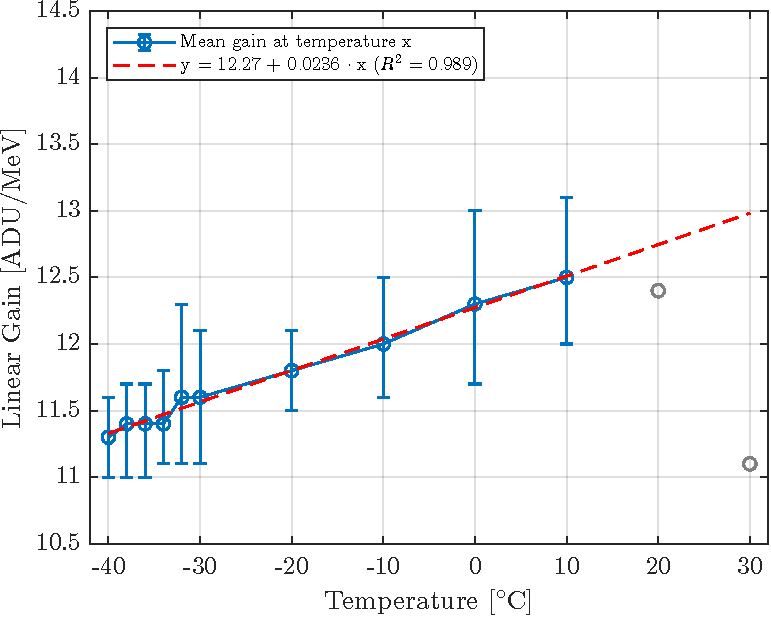
\includegraphics[width=0.475\textwidth]{Images/chap1/results/gain_pedestal/high_energy_gain_auto_0011.pdf} & 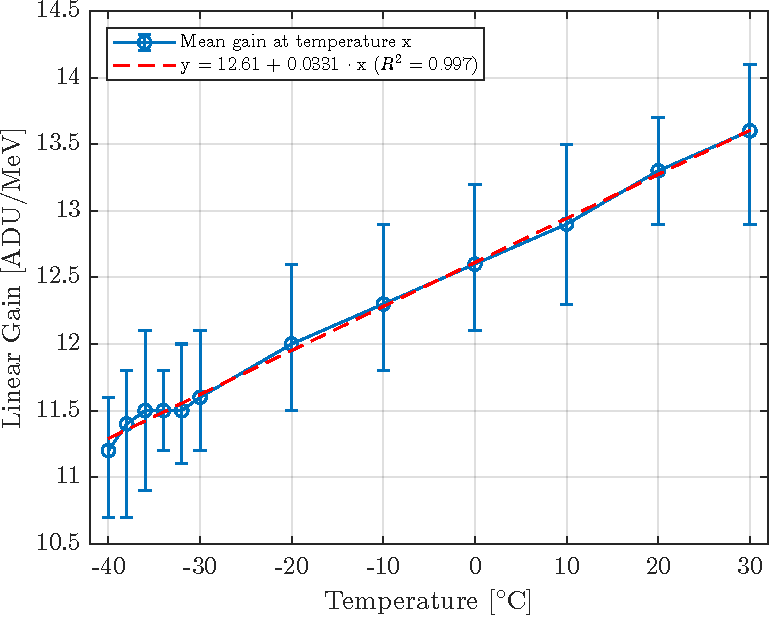
\includegraphics[width=0.475\textwidth]{Images/chap1/results/gain_pedestal/high_energy_gain_530mV.pdf}\\
    \end{tabular}
    \caption{High energy gain trend with respect to temperature from \SI{-40}{\celsius} to \SI{30}{\celsius} for automatically regulated \texttt{CSAVrefGM} voltage (on the left) and fixed to \SI{530}{\milli\volt} (on the right). The linear gain is expressed in \SI{}{ADU\per\mega\electronvolt}.}
    \label{figFDTgainHighEnergies}
\end{figure}

\noindent
It can be seen that, although $g_{0}$ assumes a value that is almost comparable between the two configurations, $g_{1}$ presents an increment of $\approx \SI{28.7}{\percent}$ when \texttt{CSAVrefGM} is set to \SI{530}{\milli\volt}, thus resulting in a higher increase in gain with respect to temperature. \hyperref[figFDTpedestalLowEnergies]{Figure \ref{figFDTpedestalLowEnergies}} and \hyperref[figFDTpedestalHighEnergies]{Figure \ref{figFDTpedestalHighEnergies}} present the trend of the pedestal as a function of temperature under the same conditions illustrated above.

% low energy pedestal
\begin{figure}[h!]
    \centering
    \begin{tabular}{cc}
        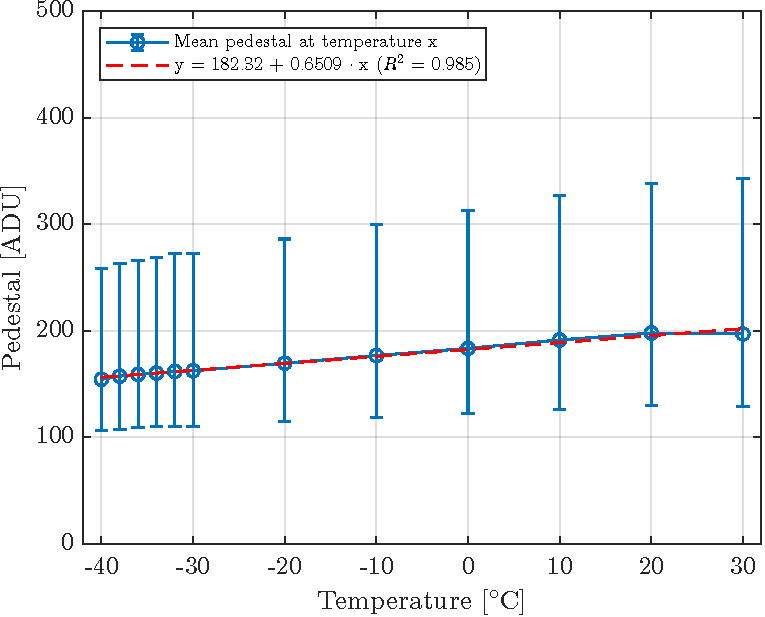
\includegraphics[width=0.475\textwidth]{Images/chap1/results/gain_pedestal/low_energy_pedestal_auto_0011.pdf} & 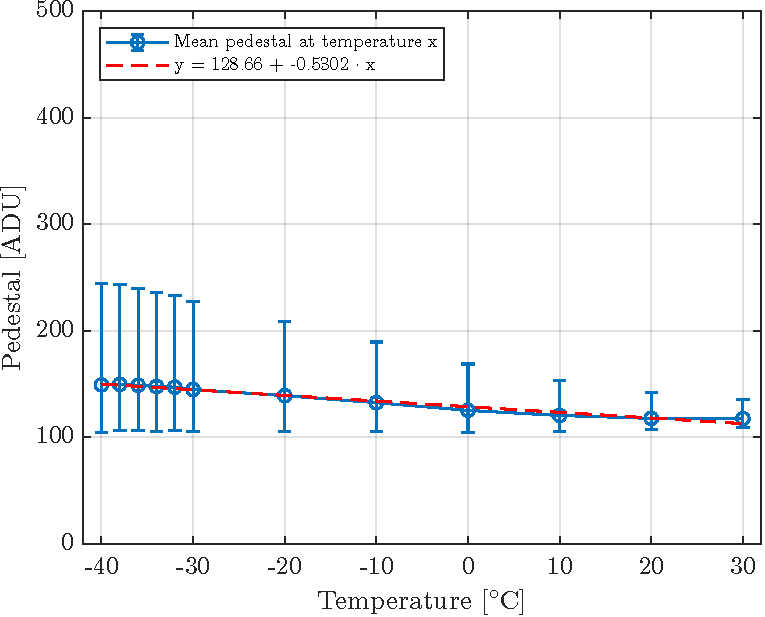
\includegraphics[width=0.475\textwidth]{Images/chap1/results/gain_pedestal/low_energy_pedestal_530mV.pdf}\\
    \end{tabular}
    \caption{Low energy pedestal trend with respect to temperature from \SI{-40}{\celsius} to \SI{30}{\celsius} for automatically regulated \texttt{CSAVrefGM} voltage (on the left) and fixed to \SI{530}{\milli\volt} (on the right).}
    \label{figFDTpedestalLowEnergies}
\end{figure}

% high energy pedestal
\begin{figure}[h!]
    \centering
    \begin{tabular}{cc}
        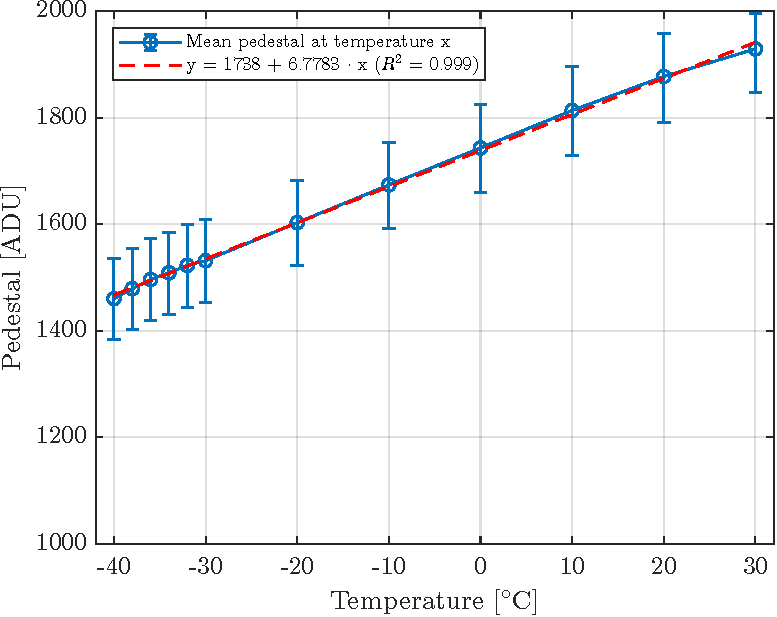
\includegraphics[width=0.475\textwidth]{Images/chap1/results/gain_pedestal/high_energy_pedestal_auto_0011.pdf} & 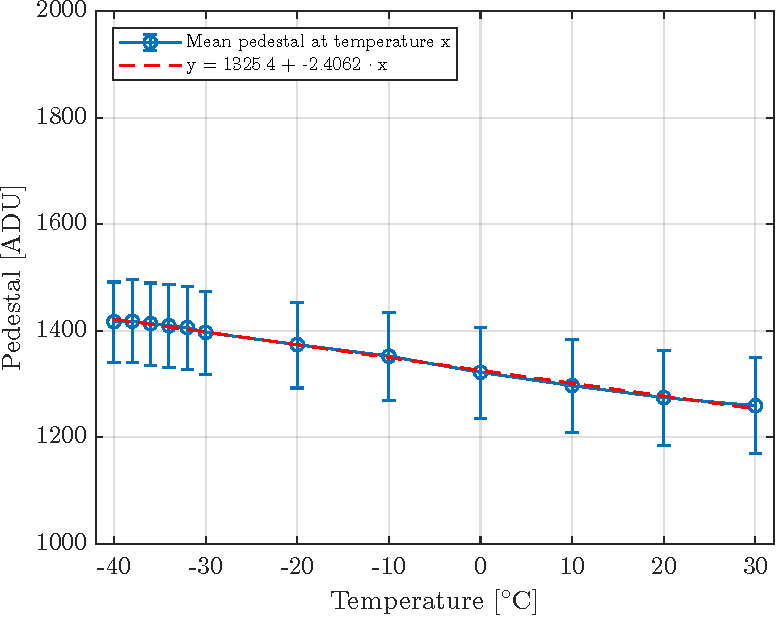
\includegraphics[width=0.475\textwidth]{Images/chap1/results/gain_pedestal/high_energy_pedestal_530mV.pdf}\\
    \end{tabular}
    \caption{High energy pedestal trend with respect to temperature from \SI{-40}{\celsius} to \SI{30}{\celsius} for automatically regulated \texttt{CSAVrefGM} voltage (on the left) and fixed to \SI{530}{\milli\volt} (on the right).}
    \label{figFDTpedestalHighEnergies}
\end{figure}

\par
Pedestal and gain measurements were used to study the variation in the position of the transfer function kink as temperature changes. In particular, \hyperref[figFDTkinkVariation]{Figure \ref{figFDTkinkVariation}} shows the interpolation curves of the transfer function in the low and high energy regions, previously referred to as \textit{X-ray} and \textit{muon} detection regions respectively. In particular, their intersection determines the point, expressed in \SI{}{\mega\electronvolt}, at which the change of slope occurs in the channel's input-output characteristic, which, in the particular example case, refers to the measurement obtained at a temperature of \SI{-40}{\celsius}. The two curves refer to the model shown in \hyperref[FDTlinearModel]{Equation \ref{FDTlinearModel}} and the resolution of the system shown in \hyperref[FDTkinkSystem]{Equation \ref{FDTkinkSystem}} allows the value of the kink at each temperature step to be determined as the intersection of the two straight lines that linearly approximate the transfer function in the high and the low energy region.

\begin{equation}
    \begin{cases}
        y = p_{LE} + g_{LE} \cdot x \\
        y = p_{HE} + g_{HE} \cdot x
    \end{cases}
    \label{FDTkinkSystem}
\end{equation}

\noindent
In particular, the subscript \textit{LE} refers to the model that describes the trend of the transfer function in the \textit{Low Energy} region, while the subscript \textit{HE} describes its trend in the \textit{High Energy} region. 

\par
Solving the system reported in \hyperref[FDTkinkSystem]{Equation \ref{FDTkinkSystem}} allows the kink value expressed in \SI{}{\mega\electronvolt} to be obtained:

\begin{equation}
    x = \frac{p_{LE} - p_{HE}}{g_{HE} - g_{LE}}
\end{equation}

\par
From the graph shown in \hyperref[figFDTkinkVariationResult]{Figure \ref{figFDTkinkVariationResult}} it is possible to appreciate the kink trend of the channel transfer function as the temperature varies, for temperature values between \SI{-40}{\celsius} and \SI{30}{\celsius}. In particular, the kink trend is shown in red when the \texttt{CSAVrefGM} voltage is fixed at \SI{530}{\milli\volt}, while it is shown in blue when this voltage is automatically varied on the basis of temperature.

\begin{figure}[h!]
    \centering
    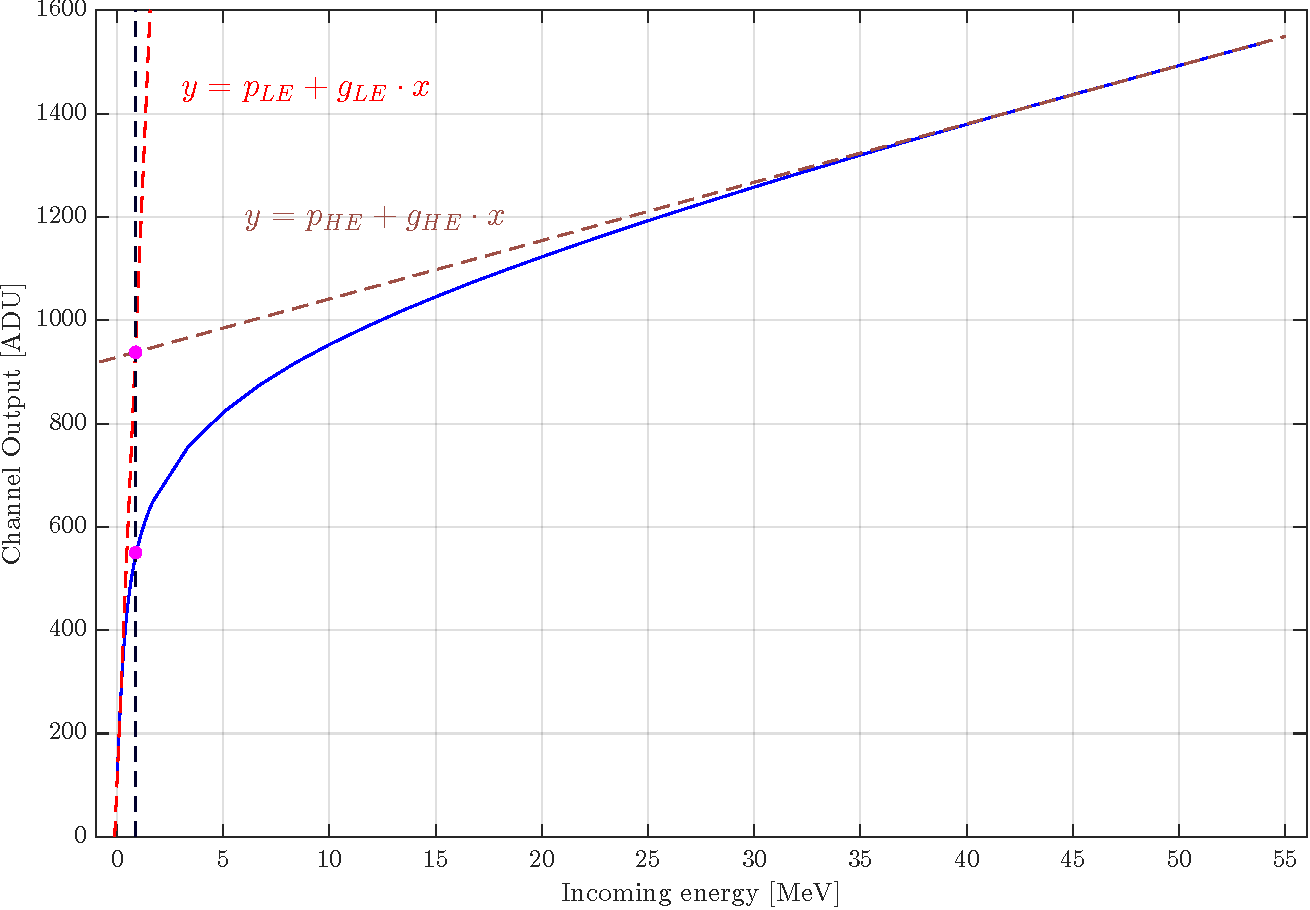
\includegraphics[width=0.65\textwidth]{Images/chap1/results/FDT/fdt_calcolo_kink.pdf}
    \caption{Method for determining the kink position: the linear models used to interpolate the transfer function in the low and high energy region are also reported.}
    \label{figFDTkinkVariation}
\end{figure}

\begin{figure}[h!]
    \centering
    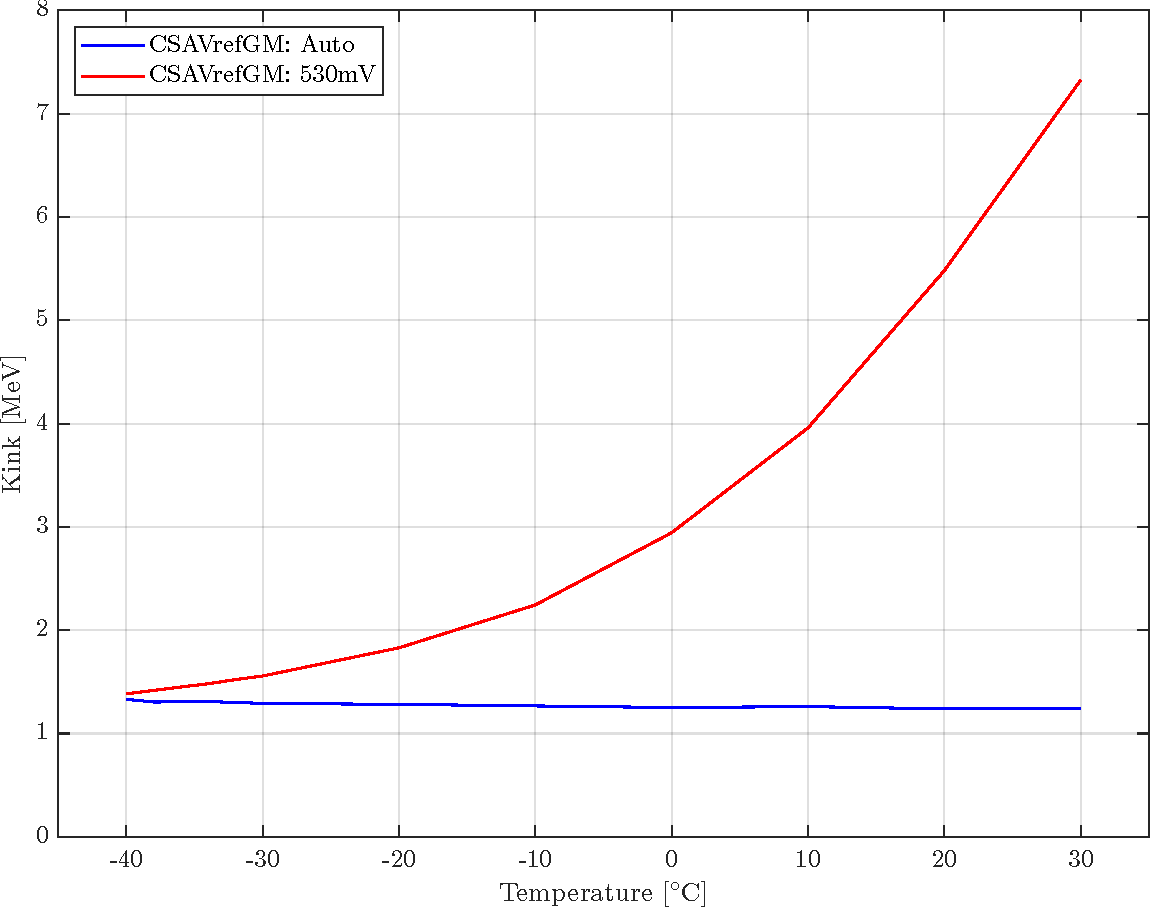
\includegraphics[width=0.55\textwidth]{Images/chap1/results/FDT/plot_pedestal_gain_auto_530mV.pdf}
    \caption{Kink behaviour as a function of temperature when \texttt{CSAVrefGM} is either fixed at \SI{530}{\milli\volt} (in red) or automatically varied as a function of temperature (in blue).}
    \label{figFDTkinkVariationResult}
\end{figure}

\par
It is easy to see that in the case where \texttt{CSAVrefGM} varies dynamically on the basis of temperature, the kink remains at an almost constant value, varying only \SI{6.95}{\percent} between \SI{-40}{\celsius} and \SI{30}{\celsius}. Conversely, in the case where this voltage is set at \SI{530}{\milli\volt} regardless of temperature, the kink undergoes a \SI{429}{\percent} variation between the two temperature extremes.


%-------------------------------------------------------------------------------
%	Global threshold voltage
%-------------------------------------------------------------------------------

\section{Global threshold voltage}
\label{thresholdVoltageANALYSIS}

This Section illustrates the measurements performed on the 8-bit DAC that provides two voltages $V_{\textit{tp}}$ and $V_{\textit{tn}}$ used by the threshold generator (described in \hyperref[secGAPSfrontend]{Appendix \ref{secGAPSfrontend}}) to generate the Signal-Over-Threshold (SOT) comparator voltage. In particular, the difference between the two voltages $\Delta V_{\textit{t}} = V_{\textit{tp}}-V_{\textit{tn}}$ is the meaningful quantity and will be referred to as \textit{global threshold voltage}: the higher $\Delta V_{\textit{t}}$, the higher the threshold of the SOT comparator. It has to be noted that the voltage $V_{\textit{tp}}$ remains constant by varying the DAC codes, whereas the voltage $V_{\textit{tn}}$ can vary from \SI{0}{\volt} to $(V_{\textit{tp}}+V_{\textit{s}})$, where $V_{\textit{s}}$ is a voltage margin which permits to obtain negative $\Delta V_{\textit{t}}$. During design of this circuit, the DAC voltage Least Significant Bit (LSB) has chosen to be

\begin{equation}
    V_{\textit{tn, LSB}} = \SI{1.2}{\milli\volt}
\end{equation}

\noindent
Since the DAC bits are 8, the maximum value of the DAC codes is $2^{8}-1$. This forces the maximum value of $V_{\textit{tn}}$ to be

\begin{equation}
    V_{\textit{tn, max}} = V_{\textit{tn, lsb}} \cdot 255 = \SI{306}{\milli\volt}
\end{equation}

\begin{figure}[ht]
    \centering 
    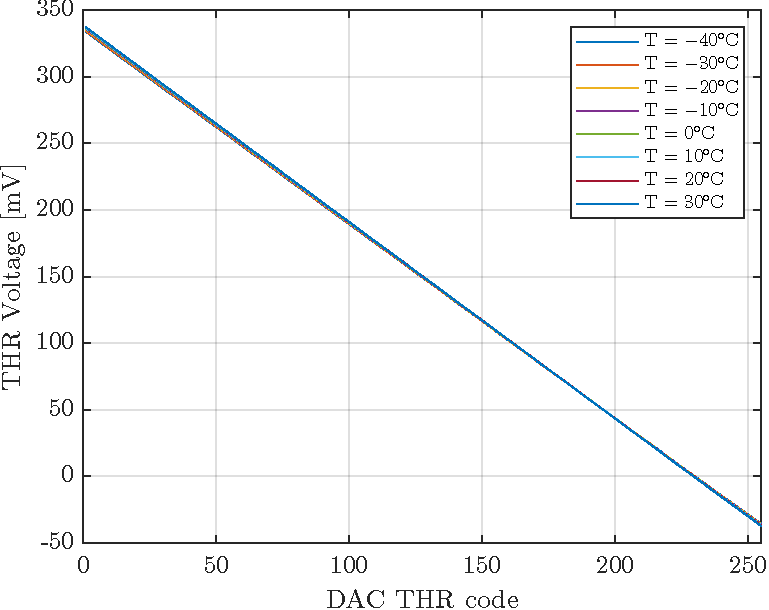
\includegraphics[width=0.63\textwidth]{Images/chap1/results/DAC_thr/DAC_thr_voltage_TEMP.pdf}
    \caption{$\Delta V_{\textit{t}}$ voltage with respect to DAC code varying temperature between \SI{-40}{\celsius} and \SI{30}{\celsius}.}
    \label{figDACthrtemp}
\end{figure}

\noindent
\hyperref[figDACthrtemp]{Figure \ref{figDACthrtemp}} shows the $\Delta V_{\textit{t}}$ voltage with respect to DAC codes varying from 0 to 255 at temperatures comprised between \SI{-40}{\celsius} and \SI{30}{\celsius} on channel 31. 

\hyperref[tabDACmaxlsb]{Table \ref{tabDACmaxlsb}} shows the maximum value assumed by $V_{\textit{tn}}$ and the corresponding DAC voltage LSB measured at each temperature. Threshold voltage measurements have been evaluated by interpolating a linear regression model, whose Equation is illustrated below. Coefficient $a$ is expressed in \SI{}{\milli\volt} and coefficient $b$ in \SI{}{\milli\volt/\celsius}. The Root Mean Square Error (RMSE) is reported for each temperature.

\begin{table}[ht]
    \centering
    \begin{tabular}{c c c} 
        \Xhline{2\arrayrulewidth}
        Temperature [\SI{}{\celsius}] & $V_{\textit{tn, max}}$ [\SI{}{\milli\volt}] & $V_{\textit{tn, lsb}}$ [\SI{}{\milli\volt}] \T\B \\
        \hline
        -40 & 333.87 & 1.45 \T\B \\
        -30 & 334.32 & 1.45 \T\B \\
        -20 & 335.35 & 1.46 \T\B \\
        -10 & 335.91 & 1.46 \T\B \\
        0 & 336.46 & 1.46 \T\B \\
        10 & 336.78 & 1.46 \T\B \\
        20 & 337.15 & 1.47 \T\B \\
        30 & 337.26 & 1.47 \T\B \\
        \Xhline{2\arrayrulewidth}
    \end{tabular}
    \caption{$V_{\textit{tn, max}}$ and $V_{\textit{tn, lsb}}$ measured at temperatures ranging from \SI{-40}{\celsius} to \SI{30}{\celsius}.}
    \label{tabDACmaxlsb}
\end{table}

\begin{equation}
    y = a + b \cdot x
\label{DAClinearmodel}
\end{equation}

\hyperref[tabDAClinearmodel1]{Table \ref{tabDAClinearmodel1}} offers a list of the model coefficients calculated over the threshold voltage measurements taken at temperatures spanning from \SI{-40}{\celsius} to \SI{30}{\celsius} along with the model RMSE.

\begin{table}[ht]
    \centering
    \begin{tabular}{c c c c} 
        \Xhline{2\arrayrulewidth}
        Temperature [\SI{}{\celsius}] & a [\SI{}{\milli\volt}] & b [\SI{}{\milli\volt/\celsius}] & RMSE \T\B \\
        \hline
        -40 & 335.12 & -1.46 & 0.15 \T\B \\
        -30 & 335.67 & -1.46 & 0.14 \T\B \\
        -20 & 336.58 & -1.46 & 0.13 \T\B \\
        -10 & 337.15 & -1.47 & 0.13 \T\B \\
        0 & 337.79 & -1.47 & 0.11 \T\B \\
        10 & 338.17 & -1.47 & 0.10 \T\B \\
        20 & 338.51 & -1.47 & 0.10 \T\B \\
        30 & 338.64 & -1.48 & 0.09 \T\B \\
        \Xhline{2\arrayrulewidth}
    \end{tabular}
    \caption{Linear regression model coefficients evaluated over global threshold measurements taken at temperatures varying from \SI{-40}{\celsius} to \SI{30}{\celsius}.}
    \label{tabDAClinearmodel1}
\end{table}

\par
\hyperref[figDACthrtemp4030]{Figure \ref{figDACthrtemp4030}} shows the global threshold voltage trend with respect to the DAC code for temperatures ranging from \SI{-40}{\celsius} to \SI{-30}{\celsius} and \SI{2}{\celsius} increments. As done previously, the global threshold voltage measurements have been evaluated by interpolating the same linear regression model described in \hyperref[DAClinearmodel]{Equation \ref{DAClinearmodel}}. The model coefficients are proposed in \hyperref[tabDAClinearmodel2]{Table \ref{tabDAClinearmodel2}}. It is immediate to see that in the \SI{-40}{\celsius} to \SI{-30}{\celsius} temperature range, the slope, $b$, of the DAC trans-characteristic remains constant with respect to temperature, while the intercept, $a$, slightly increases with an increase of temperature.

\begin{figure}[h!]
    \centering
    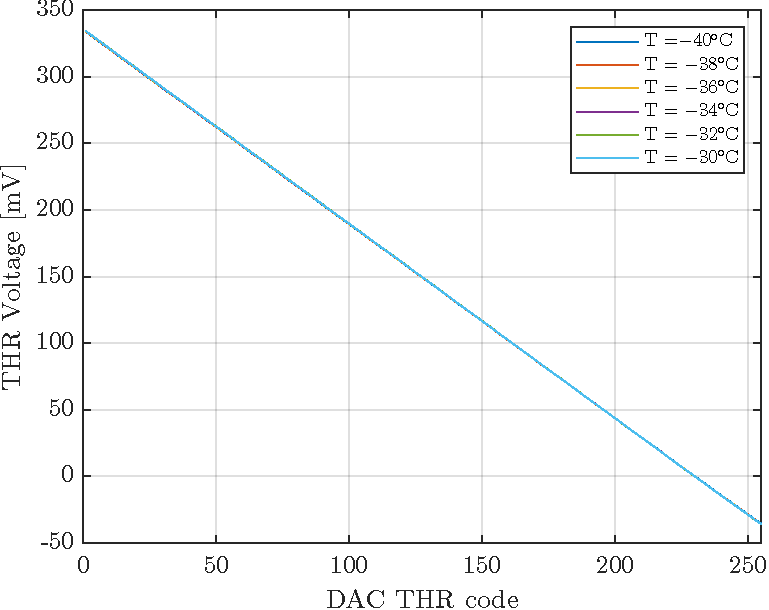
\includegraphics[width=0.63\textwidth]{Images/chap1/results/DAC_thr/DAC_thr_voltage_40-30.pdf}
    \caption{$\Delta V_{\textit{t}}$ voltage with respect to DAC code varying temperature between \SI{-40}{\celsius} and \SI{-30}{\celsius}.}
    \label{figDACthrtemp4030}
\end{figure}

\begin{table}[h!]
    \centering
    \begin{tabular}{c c c c} 
        \Xhline{2\arrayrulewidth}
        Temperature [\SI{}{\celsius}] & a [\SI{}{\milli\volt}] & b [\SI{}{\milli\volt/\celsius}] & RMSE \T\B \\
        \hline
        -40 & 335.12 & -1.46 & 0.15 \T\B \\
        -38 & 335.27 & -1.46 & 0.14 \T\B \\
        -36 & 335.50 & -1.46 & 0.14 \T\B \\
        -34 & 335.62 & -1.46 & 0.14 \T\B \\
        -32 & 335.74 & -1.46 & 0.13 \T\B \\
        -30 & 335.67 & -1.46 & 0.13 \T\B \\
        \Xhline{2\arrayrulewidth}
    \end{tabular}
    \caption{Linear regression model coefficients evaluated over global threshold measurements taken at temperatures varying from \SI{-40}{\celsius} to \SI{-30}{\celsius}.}
    \label{tabDAClinearmodel2}
\end{table}

\par
\hyperref[figDACfinethrtemp]{Figure \ref{figDACfinethrtemp}} presents the trend of the global threshold voltage with respect to the DAC code by varying the 3 bits fine threshold code on channel 31 at a constant temperature of \SI{-40}{\celsius}. As it can been appreciated in \hyperref[tabDAClinearmodel3]{Table \ref{tabDAClinearmodel3}}, the change in fine threshold code keeps the gradient unaltered while operating a shift in the DAC transfer function.

\begin{figure}[h!]
    \centering
    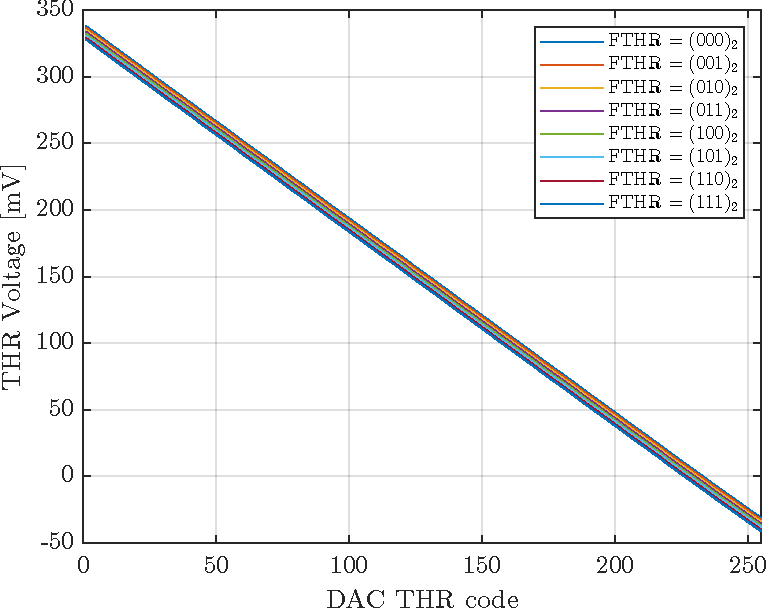
\includegraphics[width=0.63\textwidth]{Images/chap1/results/DAC_thr/DAC_thr_voltage_FTHR_-40C.pdf}
    \caption{$\Delta V_{\textit{t}}$ voltage with respect to DAC code and varying fine threshold (FTHR) code at \SI{-40}{\celsius}.}
    \label{figDACfinethrtemp}
\end{figure}

\begin{table}[h!]
    \centering
    \begin{tabular}{c c c c c} 
        \Xhline{2\arrayrulewidth}
        \multicolumn{2}{c}{FTHR} & a [\SI{}{\milli\volt}] & b [\SI{}{\milli\volt/bit}] & RMSE \T\B \\
        \hline
        0 & $(000)_{2}$ & 339.49 & -1.46 & 0.155 \T\B \\
        1 & $(001)_{2}$ & 338.10 & -1.46 & 0.152 \T\B \\
        2 & $(010)_{2}$ & 336.52 & -1.46 & 0.155 \T\B \\
        3 & $(011)_{2}$ & 335.12 & -1.46 & 0.154 \T\B \\
        4 & $(100)_{2}$ & 333.71 & -1.46 & 0.160 \T\B \\
        5 & $(101)_{2}$ & 332.22 & -1.46 & 0.156 \T\B \\
        6 & $(110)_{2}$ & 330.64 & -1.46 & 0.152 \T\B \\
        7 & $(111)_{2}$ & 329.29 & -1.46 & 0.154 \T\B \\
        \Xhline{2\arrayrulewidth}
    \end{tabular}
    \caption{Linear regression model coefficients evaluated over global threshold measurements taken by spanning the 8-bit DAC code and by varying the fine threshold (FTHR) code.}
    \label{tabDAClinearmodel3}
\end{table}


%-------------------------------------------------------------------------------
%	Equivalent Noise Charge (ENC) at -40 °C
%-------------------------------------------------------------------------------

\section{Equivalent Noise Charge (ENC) at \SI{-40}{\celsius}} \label{ENC} % -40$^{\circ}$C
The measurement of the Equivalent Noise Charge (ENC) is of fundamental importance to evaluate the performance of the channel in terms of resolution and, therefore, of minimum detectable energy. The ENC represents the electronic noise generated by the front-end channel reported in the form of equivalent noise charge at the channel input. In the case of GAPS, the main requirement for the channel comes from the resolution, that must be less than \SI{4}{\kilo\electronvolt}: this is equivalent to saying that the ENC for each channel must be less than \SI{4}{\kilo\electronvolt} in order to consider the channel suitable for the experiment.

\par
ENC is calculated by dividing the standard deviation of the noise, obtained from the pedestal measurement and measured in ADU, by the low energy gain of the channel transfer function, extracted from the input-output characteristic measurements and expressed in (ADU)/(DAC injection units):

\begin{equation}
    ENC = \frac{\sigma_{\textit{ped}} \cdot 2.35}{\mu_{\textit{ch}}} \cdot \SI{0.841}{\frac{\SI{}{\kilo\electronvolt}}{\SI{}{DAC\_inju}}} 
\end{equation}

\noindent
where $\sigma_{\textit{ped}}$ is the channel noise standard deviation and $\mu_{\textit{ch}}$ is the channel low energy gain. The \SI{0.841}{\frac{\SI{}{\kilo\electronvolt}}{\SI{}{DAC\_inju}}} value represents a conversion factor for obtaining the \SI{}{\kilo\electronvolt} measurements and it is calculated as follows:

\begin{equation}
    C_{\textit{inj}} \cdot \frac{V_{\textit{LSB, CAL}}}{\SI{0.044}{\frac{fC}{\kilo\electronvolt}}} = \SI{1.184}{\pico\farad} \cdot \frac{\SI{31.25}{\frac{\micro\volt}{DAC\_inju}}}{\SI{0.044}{\frac{fC}{\kilo\electronvolt}}} = \SI{0.841}{\frac{\kilo\electronvolt}{DAC\_inju}}
    \label{eqConversionFactor}
\end{equation}

\noindent
where $C_{\textit{inj}}$ is the injection capacitance, $V_{\textit{LSB, CAL}}$ is the LSB value of the 16-bit calibration DAC and \SI{0.044}{\frac{fC}{\kilo\electronvolt}} is the conversion factor between \SI{}{fC} and \SI{}{\kilo\electronvolt}.

\par
Lastly, 2.35 is the \textit{Fano factor}. This factor is taken into account since the ENC measurement must be expressed at Full Width at Half Maximum (FWHM). One does not simply want to consider the standard deviation of the pedestal, but the width of its Gaussian distribution at half of its maximum height. To obtain this measurement, the standard deviation of the pedestal must be multiplied by the Fano factor.

\par
\hyperref[figENCnormal]{Figure \ref{figENCnormal}} represents the ENC FWHM with and without $\SI{40}{\pico\farad}$ detector capacitors, that have been soldered on the test board and connected to the first 8 (0 to 7) channels of the ASIC in order to emulate the Si(Li) detectors capacitance. It is clear to see from the graph on the right that channels with the capacitors installed experience an increase in ENC, as it should be expected \cite{iakovidis_2018_vmm}.

\begin{figure}[ht]
    \centering
    \begin{tabular}{cc}
         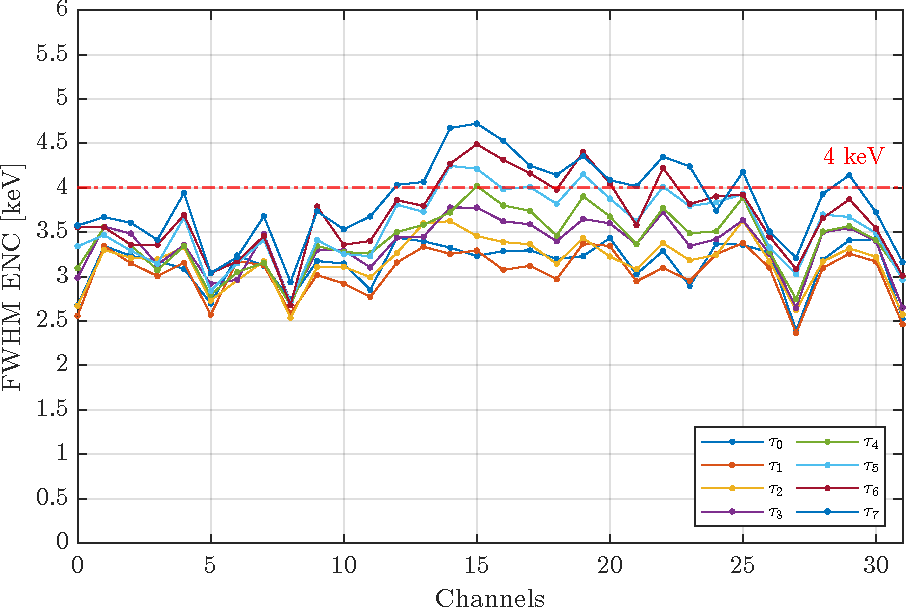
\includegraphics[width=0.475\textwidth]{Images/chap1/results/ENC_minus40C/ASIC_cold_wocaps_normal.pdf} &  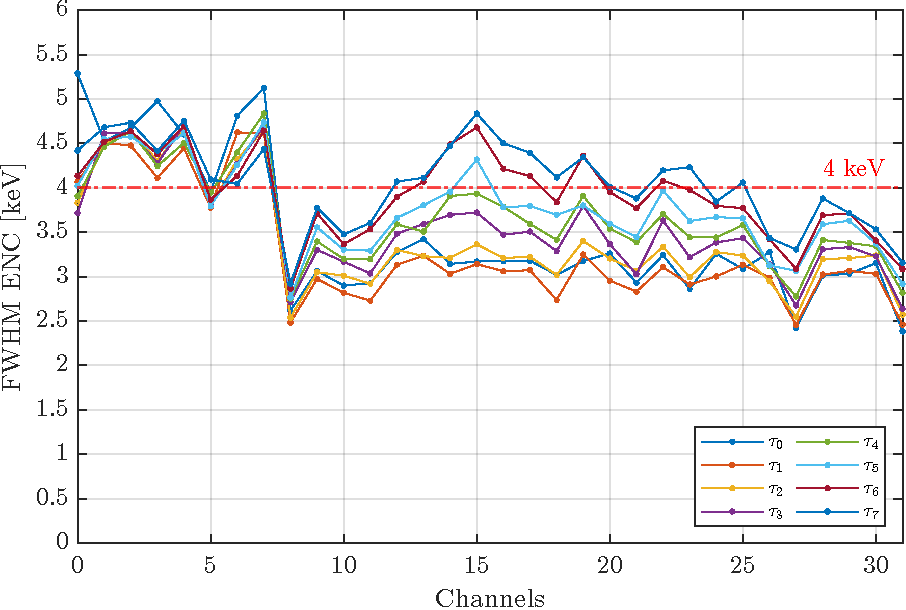
\includegraphics[width=0.475\textwidth]{Images/chap1/results/ENC_minus40C/ASIC_cold_wcaps_normal.pdf} \\
    \end{tabular}
    \caption{Graphs showing ENC FWHM without detector capacitors (on the left) and with detector capacitors (on the right) at \SI{-40}{\celsius} without removal of external interference.}
    \label{figENCnormal}
\end{figure}

\par
Since the ENC is a measurement derived from the pedestal, it is also subject to interference phenomena arising from electromagnetic noise present in the environment where the tests are performed. In this regard, a method was devised to remove interference contributions not directly attributable to pure electronic noise and the results of the analysis are presented in the following Sections.

\subsection{Sampled pedestal processing}
The pedestal is simultaneously dependent on both the channel on which the measurement is made, $y$, and the specific sample taken from the measurement, $x$, as the sum of 3 components. The first component, $p_0[y]$, represents the ideal pedestal free of external noise and interference, which therefore only depends on the specific channel on which the measurement is made. The second component, $n[x, y]$, represents the stochastic noise and the third one represents the deterministic interference component, $d[x]$. In this first analysis, the deterministic component, $d[x]$, is assumed to be common to all channels and therefore it only depends on the specific sample. For this reason, the pedestal can be written as

\begin{equation} \label{eq1}
    p[x,y] = p_0[y] + n[x, y] + d[x]
\end{equation}

\noindent
where
\begin{itemize}
    \itemsep0em 
    \item $x=1,2,...,1000$ represents the sample number.
    \item $y=0,1,...,31$ represents the channel number.
    \item $p_0$ is the ideal pedestal without noise and external interference and depends on $y$ only.
    \item $n$ is the stochastic noise component of the pedestal.
    \item $d$ is the deterministic external interference, at first we assume that it is common to all channels and it depends on $x$ only.
\end{itemize}

\subsection{Evaluation of deterministic interference}
For every sample $x$ we evaluate the mean value $p_{m}$ of the 32 channels sampled pedestal

\begin{equation} \label{eq2}
    \begin{split}
        p_m[x] & = \frac{1}{32} \sum_{y=0}^{31} p[x,y] \\
        & = \frac{1}{32} \sum_{y=0}^{31} (p_0[y] + n[x, y] + d[x]) \\
        & = p_{m, 0} + d[x]
    \end{split}
\end{equation}

\noindent
where

\begin{equation}
     \frac{1}{32} \sum_{y=0}^{31} p_0[y] = p_{m, 0}
\end{equation}

\noindent
it is due to the fact that the ideal pedestal depends entirely on the specific channel on which it is measured, so averaging the ideal pedestal over all 32 channels provides a channel-independent global average, representing the common contribution of all channels. On the other hand, it is possible to say that

\begin{equation}
     \frac{1}{32} \sum_{y=0}^{31} n[x,y] \simeq 0
\end{equation}

\noindent
and it comes from the stochastic nature of the noise, which has a constant power spectral density with respect to frequencies. This means that each frequency has the same contribution to the overall noise, thus resulting in an approximately zero average.

\par
Assuming in this first discussion that the interference contribution is common to all channels, it is easy to state that averaging the external interference $d[x]$ over the 32 channels returns the interference itself, the latter acting with the same proportion on all channels.

\begin{equation}
     \frac{1}{32} \sum_{y=0}^{31} d[x] = d[x]
\end{equation}

\subsection{Pedestal without external interference}

For every $x$ the evaluated interference is subtracted from the samples pedestal:

\begin{equation}
    \begin{split}
        p'[x,y] & = p[x,y] - p_m[x] \\
        & = p_0[y] + n[x,y] + \cancel{d[x]} - p_{m_0} - \cancel{d[x]} \\
        & = p_0[y] - p_{m_0} + n[x,y]
    \end{split}
\end{equation}

\noindent
The standard deviation with respect to $x$ of this new pedestal depends on the stochastic noise $n$ only.

\begin{figure}[h!]
    \centering
    \begin{tabular}{cc}
         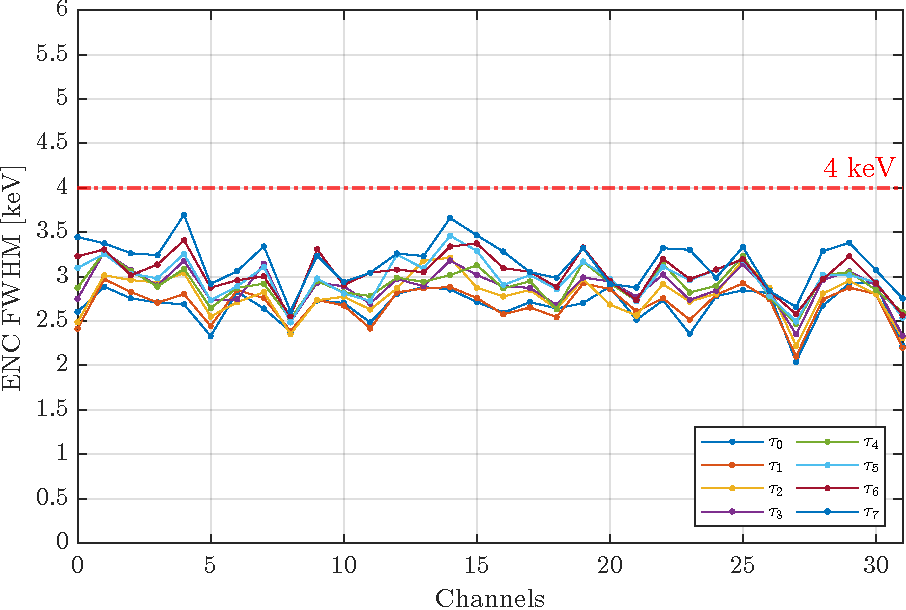
\includegraphics[width=0.475\textwidth]{Images/chap1/results/ENC_minus40C/ASIC_cold_wocaps_wo_mean.pdf} &  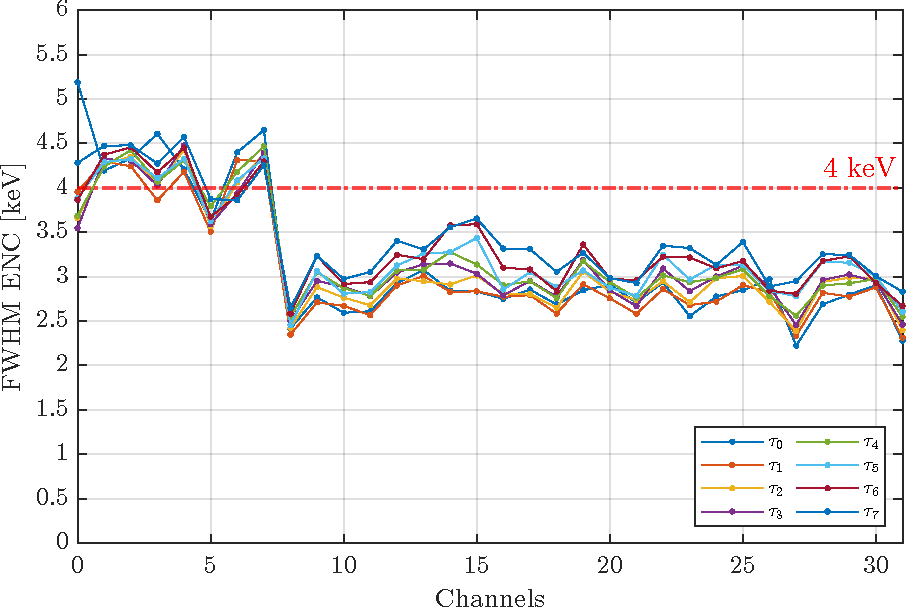
\includegraphics[width=0.475\textwidth]{Images/chap1/results/ENC_minus40C/ASIC_cold_wcaps_wo_mean.pdf} \\
    \end{tabular}
    \caption{Graphs showing ENC FWHM without detector capacitors (on the left) and with detector capacitors (on the right) at \SI{-40}{\celsius} without external interference.}
    \label{figENCwomean}
\end{figure}

\noindent
With this first method, it is therefore possible to remove the constant deterministic interference contribution, assuming to a first approximation that the disturbance acts uniformly on all 32 channels. \hyperref[figENCwomean]{Figure \ref{figENCwomean}} shows the result of the application of this first algorithm on the data shown in figure \hyperref[figENCnormal]{Figure \ref{figENCnormal}}. It is possible to appreciate the reduction of ENC, which is free of the deterministic interference component.

\subsection{Weighted external interference}
The method illustrated in this Section interprets the contribution of external deterministic interference as channel-specific, making the disturbance channel-dependent by means of a weighting factor that determines its impact, more or less marked, on the specific channel. If we assume that the same external interference $d[x]$ affects each channel with a different weight, \hyperref[eq1]{Equation (\ref{eq1})} changes as follows

\begin{equation} \label{eq3}
    p[x,y] = p_0[y] + n[x,y] + k[y] \cdot d[x]
\end{equation}

\noindent
It can be seen that the pedestal is still represented as a sum of 3 contributions, but in this case the deterministic component is weighted by means of a weight factor that determines how much the deterministic disturbance impacts on the specific channel. It goes without saying that for this method to be effective, the sample size must be sufficiently high in order to guarantee sufficiently comprehensive statistics for each individual channel. \hyperref[eq2]{Equation (\ref{eq2})} becomes

\begin{equation} \label{eq4}
    p_m[x] = p_{m_0} + k_m \cdot d[x]
\end{equation}

\noindent
where $k_m$ is the average over the 32 channels of the weight factor and can be represented as a constant factor common to all channels.

\begin{equation}
    \frac{1}{32} \sum_{y=0}^{31} k[y] \cdot d[x] = k_m \cdot d[x]
\end{equation}

\noindent
From \hyperref[eq3]{Equation (\ref{eq3})} we derive that

\begin{equation}
    d[x] = \frac{1}{k[y]} (p[x,y] - p_0[y] - n[x,y])
\end{equation}

\noindent
and therefore by replacing $d[x]$ in \hyperref[eq4]{Equation (\ref{eq4})} we obtain

\begin{equation}
    \begin{split}
        p_m[x] & = p_{m_0} + \frac{k_m}{k[y]}(p[x,y] - p_0[y] - n[x,y]) \\
        & = p_{m_0} - \frac{k_m}{k[y]} p_0[y] + \frac{k_m}{k[y]} (p[x,y] - n[x,y])
    \end{split}
\end{equation}

\noindent
By plotting $p_m[x]$ as a function of $p[x,y]$ for a given channel and by interpolating it via a linear function, the slope $m$ of the interpolating function provides the ratio between the mean channel weight $k_m$ and the weight $k[y]$ of channel $y$

\begin{equation}
    m = \frac{k_m}{k[y]}
\end{equation}

\subsection{Pedestal without weighed external interference}
As done previously, it is now necessary to remove the contribution of external deterministic interference. For this reason, for a given channel $y$ and for every sample $x$ we evaluate

\begin{equation}
    \begin{split}
        p'[x,y] & = p[x,y] - \frac{1}{m} p_m[x] \\
        & = p_0[y] + n[x,y] + k[y] \cdot d[x] - \frac{k[y]}{k_m} (p_{m_0} + k_m \cdot d[x]) \\
        & = p_0[y] + n[x,y] - \frac{k[y]}{k_m} p_{m_0} + k[y] \cdot d[x] - \frac{k[y]}{\cancel{k[m]}} \cdot \cancel{k[m]} \cdot d[x] \\
        & = p_0[y] + n[x,y] - \frac{k[y]}{k_m} p_{m_0} + \cancel{k[y] \cdot d[x]} - \cancel{k[y] \cdot d[x]} \\
        & = p_0[y] - \frac{k[y]}{k_m} \cdot p_{m_0} + n[x,y]
    \end{split}
\end{equation}

\noindent
This results in the removal of the deterministic interference component from the equation of the pedestal of each channel, reducing it entirely to the ideal contribution to which the purely stochastic component is added. Therefore, the distribution of $p'[x,y]$ depends only on the stochastic noise $n[x,y]$ for a given channel $y$.

\par
The result of the application of the latter method can be seen in \hyperref[figENCwofit]{Figure \ref{figENCwofit}}. It should be noted that, due to the limited sample size that characterises the dataset acquired during the measurements, this method is unable to provide an effective removal of the disturbance component, even resulting in a higher ENC contribution with respect to the initial one.

\begin{figure}[h!]
    \centering
    \begin{tabular}{cc}
         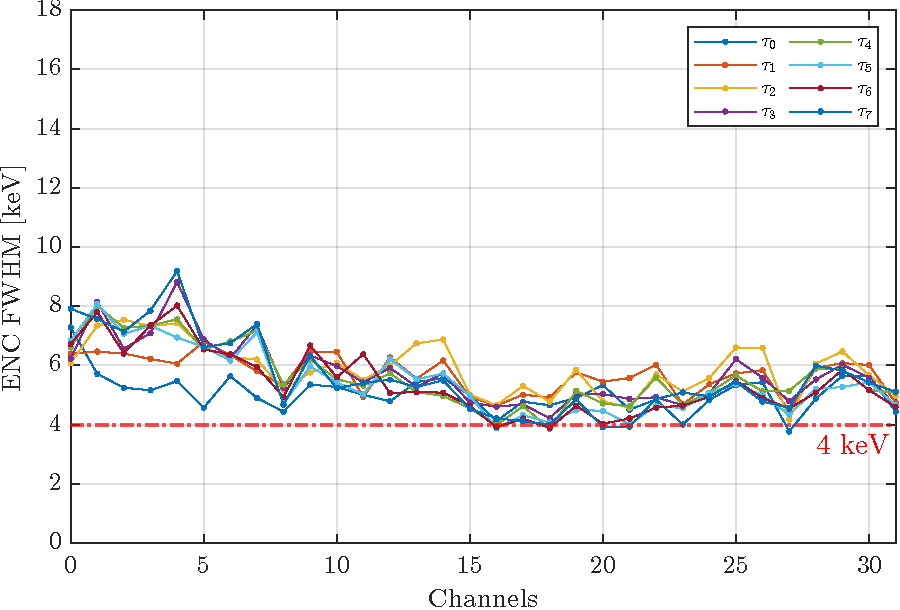
\includegraphics[width=0.475\textwidth]{Images/chap1/results/ENC_minus40C/ASIC_cold_wocaps_wo_fit.pdf} &  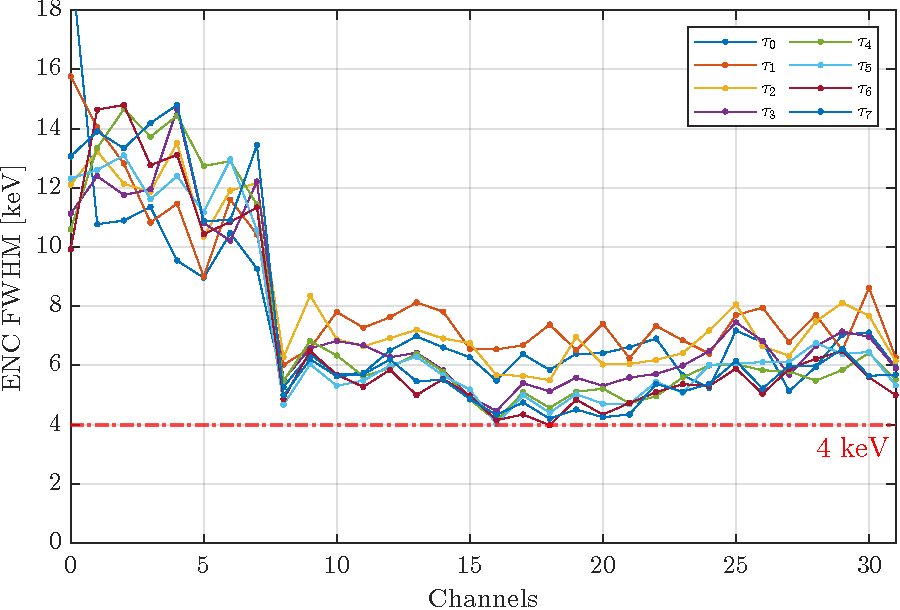
\includegraphics[width=0.475\textwidth]{Images/chap1/results/ENC_minus40C/ASIC_cold_wcaps_wo_fit.pdf} \\
    \end{tabular}
    \caption{Graphs showing ENC FWHM without detector capacitors (on the left) and with detector capacitors (on the right) at \SI{-40}{\celsius} without weighed external interference.}
    \label{figENCwofit}
\end{figure}